\documentclass[
]{thesis-ekf}
\usepackage[T1]{fontenc}
\PassOptionsToPackage{defaults=hu-min}{magyar.ldf}
\usepackage[magyar]{babel}
\usepackage{mathtools,amssymb,amsthm,pdfpages}
\usepackage{graphicx, url}
\usepackage{placeins}
\usepackage{float}
\usepackage{listings,xcolor,caption,upquote}
\footnotestyle{rule=fourth}

\newtheorem{tetel}{Tétel}[chapter]
\theoremstyle{definition}
\newtheorem{definicio}[tetel]{Definíció}
\theoremstyle{remark}
\newtheorem{megjegyzes}[tetel]{Megjegyzés}

\lstset{
	inputencoding=utf8/latin2,
	basicstyle=\footnotesize\ttfamily,
	columns=fullflexible,
	numbers=left,
	breaklines,
	postbreak=\hbox{$\mathcolor{red}{\hookrightarrow}$\ },
	xleftmargin=2cm,
	xrightmargin=2cm,
	frame=single,
	literate={á}{\'{a}}1
	{é}{\'{e}}1
	{í}{\'{i}}1
	{ó}{\'{o}}1
	{ö}{\"{o}}1
	{ő}{\H{o}}1
	{ú}{\'{u}}1
	{ü}{\"{u}}1
	{ű}{\H{u}}1
	{Á}{\'{A}}1
	{É}{\'{E}}1
	{Í}{\'{I}}1
	{Ó}{\'{O}}1
	{Ö}{\"{O}}1
	{Ő}{\H{O}}1
	{Ú}{\'{U}}1
	{Ü}{\"{U}}1
	{Ű}{\H{U}}1
}

\lstdefinestyle{myjavascript}{
	language=JavaScript,
	backgroundcolor=\color{cyan!10},
	keywordstyle=\color{blue},
	commentstyle=\itshape\color{teal},
	identifierstyle=\color{black},
	stringstyle=\color{red},
}

\lstdefinelanguage{JavaScript}{
	keywords={break, case, catch, continue, debugger, default, delete, do, else, finally, for, function, if, in, instanceof, new, return, switch, throw, try, typeof, var, void, while, with, let, const, class, export, import, extends, super},
	morekeywords={true,false,null,undefined},
	sensitive=true,
	morecomment=[l]{//},
	morecomment=[s]{/*}{*/},
	morestring=[b]",
	morestring=[b]',
	morestring=[b]`
}

\lstdefinestyle{mypython}{
	language=Python,
	basicstyle=\ttfamily\footnotesize,
	otherkeywords={self},
	keywordstyle=\color{blue}\bfseries,
	commentstyle=\color{gray}\itshape,
	stringstyle=\color{red},
	showstringspaces=false,
	tabsize=4,
	breaklines=true,
	breakatwhitespace=true,
	captionpos=b,
	escapeinside={\%*}{*\%},
	morekeywords={True,False,None}
}

\lstdefinelanguage{yaml}{
	keywords={true,false,null,y,n},
	keywordstyle=\color{blue}\bfseries,
	basicstyle=\ttfamily\small,
	sensitive=true,
	comment=[l]{\#},
	morecomment=[s]{/*}{*/},
	commentstyle=\color{gray}\ttfamily,
	stringstyle=\color{red}\ttfamily,
	morestring=[b]',
	morestring=[b]"
}

\lstdefinestyle{myyaml}{
	language=yaml,
	frame=single,
	breaklines=true,
	basicstyle=\ttfamily\small,
	keywordstyle=\color{blue}\bfseries,
	commentstyle=\color{gray}\itshape,
	stringstyle=\color{red},
	showstringspaces=false,
	tabsize=2
}

\renewcommand{\lstlistingname}{kód}

\begin{document}
	
	\institute{Matematikai és Informatikai Intézet}
	\title{Digitális személyazonosítás mesterséges intelligenciával}
	\author{Kovács Gábor\\Programtervező informatikus Bsc}
	\supervisor{Dr. Kovásznai Gergely\\Tanszékvezető, egyetemi docens}
	\city{Eger}
	\date{2025}
	\maketitle
	
	\tableofcontents
	
	\chapter*{Bevezetés}
	
	A digitalizáció és a mesterséges intelligencia fejlődése az elmúlt évtizedekben alapjaiban változtatta meg mindennapi életünket és az üzleti világ működését. Az olyan technológiák, mint a mobilalkalmazások, a felhőalapú rendszerek és a mesterséges intelligencia, lehetővé tették, hogy az információk gyorsabban és hatékonyabban legyenek elérhetők, mint valaha. Ezek a technológiák nemcsak az ipari folyamatokat, hanem a személyazonosítás és az adatkezelés területét is forradalmasították.
	
	A személyazonosítás hagyományos módszerei, mint például a papíralapú igazolványok, egyre inkább háttérbe szorulnak a digitális megoldásokkal szemben. Az e-személyi igazolványok és a biometrikus azonosítási technológiák, mint például az arcfelismerés vagy az ujjlenyomat-azonosítás, nemcsak kényelmesebbé, hanem biztonságosabbá is teszik az azonosítási folyamatokat. Az Európai Unió által bevezetett eIDAS és EUDI rendeletek is azt mutatják, hogy a digitális személyazonosítás a jövő egyik kulcsfontosságú területe.
	
	A szakdolgozat célja egy olyan mobilalkalmazás fejlesztése, amely a modern technológiák, például a React Native, az Expo, a Node.js és a MongoDB segítségével lehetővé teszi a felhasználók számára személyazonosságuk digitális igazolását. Az alkalmazás egy neurális hálózatot használ az optikai karakterfelismerés (OCR) megvalósítására, amely képes a személyi igazolványokról készült képekből kinyerni a releváns adatokat. Az így kinyert információk egy biztonságos adatbázisban kerülnek tárolásra, biztosítva a felhasználók adatainak védelmét és a rendszer megbízhatóságát.
	
	A dolgozat során bemutatom a személyazonosítás fejlődését, a digitális megoldások előnyeit és kihívásait, valamint a mesterséges intelligencia és a neurális hálók szerepét az adatfeldolgozásban. Részletesen ismertetem a projekt során használt technológiákat, a backend és frontend fejlesztési folyamatokat, valamint a rendszer tesztelését és dokumentálását. A cél egy olyan átfogó megoldás bemutatása, amely nemcsak technológiai szempontból innovatív, hanem a felhasználók számára is könnyen használható és biztonságos.\cite{projektGithub}
	
	\chapter{Személyazonosítás fejlődése és digitalizációja}
	\section{A személyi igazolványok története}
	Ebben a fejezetben röviden végigmegyünk a személyazonosító igazolványok történetén. A \emph{személyazonosítás} igénye évezredekre nyúlik vissza, hiszen a társadalmak mindig is szerették volna \emph{hiteles módon} azonosítani tagjaikat. Az ókori birodalmakban \emph{pecsétes levelek}, \emph{ujjlenyomatos agyagpecsétek} és különböző azonosító jegyek szolgáltak erre a célra. A középkorban a \emph{nemesi kiváltságokat} vagy \emph{állampolgárságot} igazoló dokumentumokat használtak, például a pápai bullákat vagy a királyi rendeleteket. \cite{okoriAzonositas, kozepkorAzonositas}
	
	A modern értelemben vett \emph{személyi igazolványok} a \emph{19. és 20. században} terjedtek el, amikor az államok egyre inkább szükségét érezték annak, hogy állampolgáraikat hivatalos dokumentumokkal azonosítsák. Magyarországon az első személyi igazolványokat a \emph{második világháború} után vezették be, és azóta számos változáson mentek keresztül, mind biztonsági, mind technológiai szempontból. \cite{magyarAzonositas}
	
	\section{A digitális azonosítás megjelenése}
	A 21. században a \emph{digitális technológia} fejlődésével a személyazonosítás egyre inkább az \emph{elektronikus rendszerekre} helyeződött át. Az internet elterjedésével növekedett az igény a \emph{biztonságos online azonosításra}, amely a hagyományos személyi igazolványok digitális megfelelőit hívta életre.
	
	Számos országban, mint például Észtországban bevezették az \emph{elektronikus személyi igazolványokat} (eID), amelyek \emph{beépített chippel} rendelkeznek, és különböző \emph{biometrikus adatokat} is tárolhatnak, mint \emph{ujjlenyomat} vagy \emph{arcfelismerési információ}. Ezek az azonosítási módszerek jelentősen javítják a biztonságot és megkönnyítik az online szolgáltatásokhoz való hozzáférést. \cite{magyarAzonositas}
	
	\section{A mobiltechnológia és az azonosítás}
	Az \emph{okostelefonok} és a \emph{mobilalkalmazások} terjedésével az azonosítás folyamata tovább egyszerűsödött. A felhasználók ma már egyetlen kattintással vagy \emph{biometrikus azonosítással} (pl. \emph{Face ID}, \emph{ujjlenyomat-olvasó}) hitelesíthetik magukat különböző szolgáltatásokhoz.
	
	A \emph{mobiltechnológia} lehetővé tette a digitális személyazonosítás gyorsabb, kényelmesebb és biztonságosabb formáit. A \emph{blockchain}\footnote{Az adatok ,,blokkokba'' vannak tárolva, amelyek egymáshoz vannak láncolva, így egy folyamatos, biztonságos láncot alkotnak.} alapú azonosítási rendszerek pedig tovább fokozzák az \emph{adatok védelmét}, lehetőséget adva a felhasználóknak, hogy nagyobb kontrollt gyakoroljanak személyes adataik felett.
	
	\section{A digitalizáció jövője a személyazonosításban}
	A jövőben a személyazonosítás módszerei tovább fejlődnek, egyre inkább az \emph{automatizált} és \emph{AI-alapú rendszerek} irányába. Az \emph{arcfelismerés}, a \emph{hangalapú azonosítás} egyre népszerűbbé válik.
	
	A digitális személyazonosítás előnye, hogy \emph{gyorsabb} és \emph{hatékonyabb} az offline módszereknél, ugyanakkor komoly \emph{adatbiztonsági kihívásokat} is felvet. A jövő fejlesztései során kulcsfontosságú lesz a \emph{magánszféra védelme} és az \emph{etikus adatkezelés} biztosítása.
	
	A \emph{digitális személyi igazolványok} az állampolgárok azonosításának egyre népszerűbb eszközei világszerte. Ezek az okmányok nemcsak a hagyományos, fizikai igazolványok elektronikus megfelelői, hanem további funkciókkal is rendelkezhetnek, például \emph{online hitelesítésre}, \emph{elektronikus aláírásra} vagy egyes állami és magánszolgáltatások elérésére.
	
	Bár a digitális személyazonosítás rengeteg \emph{előnyt} kínál, számos \emph{kihívás} is társul hozzá, amelyek megoldása kulcsfontosságú a széleskörű elterjedéshez.

	\section{Előnyök}
	A \emph{digitális személyi igazolványok} lehetővé teszik az azonosítás és hitelesítés \emph{gyors} és \emph{kényelmes} módját. Az állampolgárok anélkül igazolhatják magukat, hogy fizikai okmányt kellene magukkal hordaniuk, hiszen az azonosító adatok tárolhatók egy \emph{mobiltelefonon} vagy egy \emph{biztonságos szerveren}. Magyarországon a DÁP\footnote{Digitális Állampolgárság Program} valósítja ezt meg.
	
	Például egy \emph{e-személyi igazolvány} segítségével egy banki ügyintézés vagy egy online regisztráció néhány kattintással elvégezhető, míg a hagyományos személyazonosítás esetében papírokat kell kitölteni, aláírni és személyesen bemutatni.
	
	A digitális személyazonosító igazolványok a legmodernebb \emph{titkosítási technológiákat} alkalmazzák, így \emph{nehezebben hamisíthatók}, mint a hagyományos plasztikkártyák. Egy jól megtervezett digitális rendszerben az adatok ellenőrzése és tárolása \emph{szigorú biztonsági szabványok} szerint történik, csökkentve az illetéktelen hozzáférés vagy visszaélés esélyét. Az Európai Unióban az Európai Bizottság felelős a digitális személyazonosításra vonatkozó szabályozásért, melynek keretében az \emph{eIDAS} és az \emph{EUDI} rendeletek meghatározó szerepet töltenek be a biztonságos digitális azonosítási keretrendszer kialakításában. \cite{eIDAS, EUDI}
	
	\emph{Biometrikus azonosítókkal} (például \emph{arcfelismerés} vagy \emph{ujjlenyomat}) kombinálva az e-személyik még biztonságosabbá válhatnak, hiszen a felhasználó azonosítása egyértelmű és nehezen másolható.\cite{bioMetricsFuture}
	
	A digitális személyi igazolványok hozzájárulhatnak a \emph{papíralapú ügyintézés csökkentéséhez}, ami nemcsak a \emph{környezetvédelmet} szolgálja, hanem a közigazgatási rendszerek \emph{hatékonyságát} is növeli. A kevesebb nyomtatás, postázás és manuális adatfeldolgozás hosszú távon jelentős \emph{költségmegtakarítást} eredményezhet az állam és a vállalatok számára is.
	
	\section{Kihívások}
	A digitális személyazonosító rendszerek egyik legnagyobb kihívása az \emph{adatbiztonság}. Mivel ezek az igazolványok személyes adatokat tartalmaznak, kiemelt célpontjai lehetnek \emph{kibertámadásoknak} és \emph{adatlopásoknak}. Egy esetleges rendszerfeltörés vagy adatvédelmi incidens súlyos következményekkel járhat az érintettek számára.
	
	Ennek elkerülése érdekében olyan technológiákat kell alkalmazni, mint a \emph{többfaktoros hitelesítés}, az adatok \emph{titkosítása} és a \emph{decentralizált adattárolás}. Az \emph{adatvédelmi jogszabályok} is szigorúan szabályozzák, hogy a digitális személyi igazolványokhoz kapcsolódó információkat hogyan lehet kezelni és tárolni.
	
	Bár a digitális személyi igazolványok kényelmesek lehetnek a technológiailag fejlett országokban, nem mindenki fér hozzá megfelelő eszközökhöz vagy internetkapcsolathoz. Az \emph{idősebb generációk}, a \emph{technológiai ismeretekkel kevésbé rendelkezők} vagy a \emph{hátrányos helyzetű régiókban élők} számára nehézséget jelenthet az új rendszer használata.
	
	Emellett az \emph{infrastruktúrának} is fel kell készülnie a digitális személyazonosítás kezelésére. Például egy digitális személyi igazolvány csak akkor használható széles körben, ha az intézmények és vállalkozások rendszerei \emph{kompatibilisek} vele.
	
	A digitális azonosítás \emph{jogi szabályozása} még sok helyen gyerekcipőben jár. Az \emph{eltérő nemzeti szabályozások} és az adatvédelmi törvények miatt nehéz olyan \emph{univerzális rendszert} kialakítani, amely minden országban elfogadott és kompatibilis lenne a helyi előírásokkal.
	
	Például egy olyan digitális személyi igazolvány, amely egy adott országban teljes körű hitelesítésre képes, nem biztos, hogy egy másik országban is elfogadott. A \emph{nemzetközi standardok} és \emph{együttműködések} kialakítása kulcsfontosságú lehet a rendszer globális elterjedése szempontjából.
	
	\chapter{A mesterséges intelligencia szerepe az adatfeldolgozásban}
	A \emph{mesterséges intelligencia} (MI) forradalmasította az adatfeldolgozást és az automatizált döntéshozatalt. A hagyományos, manuális adatrögzítési módszerekkel szemben az MI-alapú rendszerek képesek \emph{nagy mennyiségű információ} \emph{gyors} és \emph{pontos} feldolgozására, ami különösen hasznos a dokumentumok digitalizálása és azonosítási rendszerek fejlesztése terén.
	
	\section{Mi az az OCR (Optikai karakterfelismerés)?}
	Az \emph{Optical Character Recognition} (OCR) egy olyan technológia, amely képes nyomtatott vagy kézírásos szövegeket \emph{digitális formátumba} alakítani. Az OCR segítségével a dokumentumokról készült fényképeken található szöveg \emph{gépileg olvasható} formátummá konvertálható, így az adatok feldolgozása és tárolása \emph{automatizálható}.
	
	Az OCR működésének lépései: \begin{enumerate} \item \textbf{Kép előfeldolgozása} -- A képből eltávolítják a \emph{zajokat} (például árnyékokat vagy torzításokat), hogy a karakterek élesebben felismerhetők legyenek. \item \textbf{Karakterek felismerése} -- Az MI-alapú OCR rendszerek általában \emph{neurális hálók} segítségével azonosítják az egyes betűket és számokat. \item \textbf{Szöveg átalakítása és értelmezése} -- A felismerés után a szöveget \emph{szerkezetileg elemzik}, hogy a megfelelő adatokat lehessen kinyerni belőle (például név, születési dátum, igazolványszám). \end{enumerate}
	
	Az ilyen rendszerek \textbf{\emph{gépi tanulással}} folyamatosan fejleszthetők: minél több dokumentumot dolgoznak fel, annál pontosabb lesz a felismerés és az adatkinyerés.
	
	\section{Hogyan segíthet az MI a dokumentumok feldolgozásában?}
	A mesterséges intelligencia a dokumentumfeldolgozás több aspektusában is jelentős segítséget nyújt: \begin{itemize} \item \textbf{\emph{Automatizált adatkinyerés}} -- Az MI-alapú rendszerek az igazolványokról gyorsan és pontosan kivonják az adatokat, csökkentve a manuális bevitel szükségességét. \item \textbf{\emph{Hibajavítás és adatellenőrzés}} -- Az MI képes felismerni és javítani a karakterfelismerési hibákat, valamint ellenőrizni az adatok érvényességét (pl. egy születési dátum valós lehet-e). \item \textbf{\emph{Biztonsági ellenőrzések}} -- Az MI algoritmusok kiszűrhetik a hamis vagy manipulált igazolványokat azáltal, hogy összehasonlítják azokat ismert mintákkal és adatbázisokkal. \item \textbf{\emph{Adatvédelmi és titkosítási megoldások}} -- Az MI segítségével érzékeny személyes adatok anonim módon tárolhatók és dolgozhatók fel, csökkentve az adatlopás kockázatát. \end{itemize}
	
	\section{A mesterséges intelligencia jövője az adatfeldolgozásban}
	Ahogy az MI-technológiák egyre fejlettebbé válnak, az adatfeldolgozás pontossága és hatékonysága tovább javulhat. A jövőben várható fejlesztések közé tartozik: \begin{itemize} \item \textbf{\emph{Még pontosabb OCR és természetes nyelvfeldolgozás}} (NLP) -- Az MI képes lesz még bonyolultabb dokumentumokat is pontosan értelmezni. \item \textbf{\emph{Valós idejű adatfeldolgozás}} -- Az azonosítási folyamatok azonnali ellenőrzése és feldolgozása még gyorsabbá válhat. \item \textbf{\emph{Blokklánc és decentralizált identitáskezelés}} -- Az MI és a blokklánc kombinálásával a személyazonosító adatok még biztonságosabbá tehetők. \end{itemize}
	
	Összességében a mesterséges intelligencia egyre fontosabb szerepet tölt be a személyazonosító dokumentumok \emph{digitális feldolgozásában}. Az \emph{automatizálás}, a \emph{pontosság} és a \emph{biztonság} növelésével hozzájárul ahhoz, hogy a felhasználók kényelmesebben és gyorsabban intézhessék ügyeiket a digitális világban.

\chapter{Neurális hálók}
A \emph{mély neurális hálózatok} több egymásra épülő rétegből állnak, amelyek \emph{mesterséges neuronokat} vagy \emph{csomópontokat} tartalmaznak. \Aref{fig-neural} ábrán szemléltetett módon ezek a csomópontok különböző \emph{matematikai műveleteket} végeznek el, jellemzően \emph{lineáris transzformációkat}, amelyek révén az információ feldolgozása és továbbítása történik.

\begin{figure} \centering 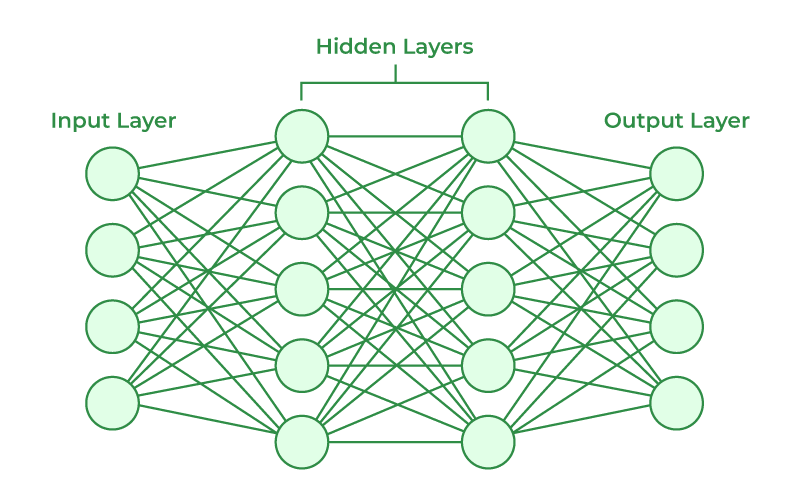
\includegraphics[width=10cm]{Neural-Networks-Architecture} \caption{Neurális háló, forrás: \cite{neuralNetworkImage}} \label{fig-neural} \end{figure}

Ezek a hálózatok három fő rétegből épülnek fel: a \emph{bemeneti rétegből}, a \emph{rejtett rétegekből} és a \emph{kimeneti rétegből}. Az első réteg, a bemeneti réteg, fogadja és előkészíti az adatokat, amelyeket aztán a rendszer a következő szintek felé továbbít. A köztes rétegek, az úgynevezett rejtett rétegek, az adatok feldolgozását végzik. Ezek a rétegek az információkat \emph{nemlineáris aktivációs függvények} segítségével alakítják át, és fokozatosan kinyerik a releváns jellemzőket a bemenetekből. \cite{neuralNetwork}

A rejtett rétegek működése közvetlenül nem megfigyelhető, mivel a bennük található paraméterek – azaz a \emph{súlyok} és \emph{eltolások} – a \emph{tanulási folyamat} során finomhangolódnak. Ezek a paraméterek lehetnek kezdetben véletlenszerűek, de előfordulhat, hogy előre meghatározott értékekkel indulnak, amelyeket korábbi tanulási tapasztalatok alapján állítottak be. A rejtett rétegek célja, hogy az adatok \emph{összetett mintázatait} felismerjék és olyan jellemvonásokat azonosítsanak, amelyek hozzájárulnak a végső döntések meghozatalához, például egy predikció vagy osztályozás formájában. \cite{neuralNetwork}

A rejtett rétegek által előállított információ végül eljut a kimeneti réteghez, amely a hálózat végső eredményeit biztosítja. Az adott feladattól függően ez a réteg lehetővé teszi az \emph{osztályozást}, \emph{előrejelzést} vagy akár új minták generálását. Az adatok ilyen módon történő feldolgozását és továbbítását \emph{előreterjesztésnek} nevezzük, amely \aref{fig-neural}. ábrán is szemléltetett módon zajlik. \cite{neuralNetwork}

\section{TensorFlow – A Mélytanulási Keretrendszer}
A \emph{TensorFlow} egy nyílt forráskódú, fejlett \emph{gépi tanulási} és \emph{mesterséges intelligencia} (AI) keretrendszer, amelyet a Google fejlesztett ki és tett elérhetővé 2015-ben. Az egyik legnépszerűbb eszközként szolgál a mesterséges intelligencia alkalmazások fejlesztésében, különösen a \emph{mélytanulási modellek} létrehozásában. A TensorFlow egy olyan rugalmas és hatékony platform, amely lehetővé teszi a kutatók és fejlesztők számára, hogy széleskörű gépi tanulási modelleket és alkalmazásokat hozzanak létre és futtassanak különböző környezetekben, beleértve a \emph{felhőt}, a \emph{mobil eszközöket} és a \emph{beágyazott rendszereket}. \cite{tensorflowDocs}

A TensorFlow kifejlesztésének fő célja, hogy megkönnyítse a gépi tanulási modellek létrehozását és implementálását, ugyanakkor a számítási feladatokat egy \emph{skálázható}, \emph{párhuzamosítható} grafikus számítási modellben kezelje. Az eszközt eredetileg a Google Brain csapata készítette, hogy támogassa a Google-hoz tartozó projektek, például a keresőoptimalizálás, képfeldolgozás, gépi fordítás, és más mesterséges intelligencia alkalmazások fejlesztését. \cite{tensorflowDocs}

A TensorFlow támogatja a különböző gépi tanulási algoritmusokat, mint például a \emph{felügyelt} és \emph{felügyelet nélküli tanulás}, valamint a mélytanulás különböző típusait, mint a neurális hálózatok, \emph{konvolúciós neurális hálózatok} (CNN) és \emph{,,ismételd'' neurális hálózatok} (RNN). A TensorFlow képes hatékonyan futtatni modelleket \emph{CPU}-n, \emph{GPU}-n és más dedikált hardvereken, mint például a \emph{Tensor Processing Unit} (TPU), amely a Google által kifejlesztett egyedi hardver az AI számítási feladatok gyorsítására. \cite{tensorflowDocs}

A TensorFlow egyik legnagyobb előnye az, hogy skálázható, tehát képes kis mértékű alkalmazásoktól kezdve, a világ legnagyobb felhőalapú rendszereit is kiszolgálni. Emellett a TensorFlow lehetővé teszi a modellek mobil eszközökön való futtatását, így a fejlesztők egyszerűen vihetik a mélytanulási megoldásaikat a mobil alkalmazások világába is. \cite{tensorflowDocs}

\section{Konvolúciós neurális hálózatok és a Keras könyvtár}
A \emph{konvolúciós neurális hálózatok} (CNN-ek) a mélytanulás egyik leggyakrabban alkalmazott architektúrái, különösen \emph{képfeldolgozási} feladatokban. Felépítésük a vizuális információk feldolgozására lett optimalizálva, így kiválóan alkalmazhatók például \emph{arcfelismerésre}, \emph{nem-} és \emph{korosztály-becslésre}, vagy más \emph{biometrikus minták} feldolgozására. \cite{cnnFoundations}

A CNN-ek működésének alapja a \emph{konvolúciós réteg}, amely képes a bemeneti képekről \emph{jellemzőket} (éleket, mintázatokat, textúrákat stb.) kinyerni úgy, hogy a teljes képet nem kell egydimenziós vektorrá alakítani, hanem \emph{lokális régiókat} vizsgál. Ezután általában következik egy \emph{pooling réteg}, amely az adatok térbeli méretét csökkenti, miközben a legfontosabb jellemzőket megtartja. \cite{deepLearningBook}

A klasszikus \emph{teljesen összekötött rétegek} (fully connected layers) csak a feldolgozás legvégén jelennek meg, amikor már a rendszer „megtanulta", hogy milyen tulajdonságokat fontos figyelembe venni. A tanítás során a CNN megtanulja azokat a \emph{szűrőket}, amelyek a feladat szempontjából releváns mintázatokat emelik ki. \cite{faceDetection}

A CNN-ek használata különösen előnyös olyan esetekben, amikor az adatok erősen vizuális természetűek, például arc- vagy dokumentumképek, amelyeket az alkalmazás is feldolgoz. A hálózatok képesek tanulni a bemenetekből kiolvasható jellemzőket, így automatikusan felépíthetnek egy hatékony osztályozási logikát. \cite{cvAndDL}

A CNN-ek implementálásához az egyik leggyakrabban használt eszköz a \textbf{\emph{Keras}}, amely a TensorFlow magas szintű API-jaként működik. A Keras \emph{deklaratív stílusban} teszi lehetővé a modellek gyors és egyszerű definiálását, betanítását és értékelését, így különösen alkalmas \emph{prototípus-készítésre}, mobilalkalmazásokhoz való modellek fejlesztésére, vagy oktatási célokra. \cite{kerasGuide}

A dolgozatban bemutatott alkalmazás fejlesztése során is használatra került a Keras, amelynek segítségével könnyedén létre lehetett hozni a konvolúciós rétegekből és teljesen összekapcsolt (dense) rétegekből álló hálózatot, valamint alkalmazni lehetett az \emph{Adam optimalizáló algoritmust} is, amely gyors és stabil tanulást biztosít. \cite{adamOptimizer}
\chapter{Backend-en használt technológiák}
\section{Node.js}
A \emph{backend fejlesztés} kulcsszerepet játszik a modern web- és mobilalkalmazások működésében, hiszen ezen a rétegen történik az \emph{adatok kezelése}, \emph{tárolása} és \emph{kiszolgálása}. A szerveroldali technológiák közül a \emph{Node.js} az egyik legnépszerűbb választás, amely lehetőséget biztosít arra, hogy az alkalmazás teljes fejlesztése \emph{JavaScript} nyelven történjen. A Node.js egy gyors és hatékony futtatókörnyezet, amely \emph{eseményvezérelt} és \emph{nem blokkoló} működésének köszönhetően különösen alkalmas nagy teljesítményt igénylő alkalmazások készítésére.

\subsection{A Node.js alapjai és működési modellje}
A Node.js a \emph{Google V8 JavaScript motorjára} épül, amely lehetővé teszi a JavaScript kód gyors végrehajtását szerveroldalon. Az egyik legfontosabb sajátossága az \emph{aszinkron} és eseményvezérelt működés, amely lehetővé teszi, hogy a szerver egyszerre több kérést is kezeljen anélkül, hogy az egyes műveletek blokkolnák egymást. Mivel a Node.js nem használ többszálú feldolgozást, hanem \emph{egyetlen szálon} fut, a skálázhatóságot egy úgynevezett \emph{eseményhurok} biztosítja, amely a beérkező kéréseket folyamatosan fogadja és kezeli. \cite{tilkovNode}

Az aszinkron működés egyik alapvető eszköze a \emph{visszahívási függvények} (callback), amelyeket később az \emph{ígéretek} (Promises) és az \emph{async/await} konstrukciók egészítettek ki.

\subsection{A Node.js előnyei és kihívásai}
A Node.js egyik legnagyobb előnye a \emph{teljesítménye} és \emph{skálázhatósága}. Az eseményvezérelt architektúra miatt a szerver könnyedén kezelhet nagy számú \emph{egyidejű kapcsolatot} anélkül, hogy túlterhelődne. Ez különösen előnyös olyan alkalmazások esetében, amelyek \emph{valós idejű interakciót} igényelnek, például csevegőalkalmazások vagy élő adatstreaming megoldások.

Egy másik fontos előny a JavaScript használata mind a \emph{frontend}, mind a \emph{backend} fejlesztés során. Ez lehetővé teszi, hogy a fejlesztőcsapatok egységes technológiai környezetben dolgozzanak, ami jelentősen csökkenti a fejlesztési időt és egyszerűsíti a kód karbantarthatóságát.

A Node.js azonban nem minden esetben ideális választás. A \emph{CPU-intenzív műveletek}, például nagy mennyiségű számítási feladatokat végző algoritmusok vagy mesterséges intelligencia modellek futtatása esetén a Node.js teljesítménye korlátozott lehet. Mivel egyszálú környezetben működik, a nagy számítási igényű feladatok blokkolhatják az egész szerver működését. Ilyen esetekben érdemes \emph{külső szolgáltatásokat} vagy \emph{külön szálakon futó háttérfolyamatokat} használni a terhelés elosztására.

\subsection{Backend fejlesztés Express.js segítségével}
A Node.js önmagában is alkalmas szerverek létrehozására, de a fejlesztést jelentősen megkönnyíti az \emph{Express.js}, amely egy minimalista és rugalmas webkeretrendszer. Az Express lehetőséget biztosít \emph{API végpontok} kialakítására, \emph{HTTP kérések} kezelésére és \emph{middleware-ek} használatára. \cite{nodeInAction, holmesExpress}

\subsection{Adatbázis-kezelés Node.js-ben}
A backend fejlesztés egyik alapvető feladata az \emph{adatkezelés}, amelyhez különböző adatbázisokat lehet használni. A Node.js kompatibilis mind a \emph{relációs (SQL)}, mind a \emph{NoSQL} adatbázisokkal. A relációs adatbázisok, például a \emph{MySQL} vagy a \emph{PostgreSQL} strukturált adatkezelést biztosítanak, míg a NoSQL megoldások, mint a \emph{MongoDB}, rugalmasabb adatmodellezést tesznek lehetővé.

Egy MongoDB alapú adatbázis kapcsolat létrehozására a \emph{Mongoose} csomag használható, amely egy \emph{objektumorientált adatmodellezést} biztosító eszköz. A Mongoose használata lehetővé teszi az adatbázis-interakciók egyszerű kezelését, miközben biztosítja az adatok \emph{validálását} és \emph{strukturálását}. Az objektumorientált modellnek köszönhetően a JavaScript objektumok könnyedén átalakíthatók adatbázis-bejegyzésekké. \cite{mongooseDocs}

\section{MongoDB}
A \emph{MongoDB} egy \emph{nyílt forráskódú}, \emph{dokumentum-orientált adatbázis-kezelő rendszer} (DBMS), amelyet a MongoDB, Inc. fejlesztett. Az adatokat \emph{dokumentumok} formájában tárolja, amelyek általában \emph{JSON-szerű BSON} formátumban (Binary JSON) kerülnek mentésre. Ez lehetővé teszi, hogy az adatokat \emph{rugalmasan}, \emph{skálázható} módon tároljuk, így ideális választás \emph{nagy mennyiségű}, \emph{változó szerkezetű} adat kezelésére.

A MongoDB-t 2007-ben alapították, és gyorsan elnyerte a fejlesztők és cégek körében a népszerűséget a hagyományos relációs adatbázisokkal szembeni előnyei miatt. Mivel a MongoDB nem követeli meg a \emph{szigorú séma} használatát, az adatokat szabadon, dinamikusan tárolhatjuk, amely különösen hasznos a gyorsan változó vagy nem strukturált adatokkal dolgozó alkalmazások számára.

A MongoDB-t széles körben használják különböző típusú alkalmazásokban, beleértve a \emph{webalkalmazásokat}, \emph{analitikai platformokat}, valamint a \emph{Big Data} és a \emph{gépi tanulási} megoldásokat is. A NoSQL adatbázisok közé tartozik, amelyek az újabb alkalmazásfejlesztési igényeknek megfelelően nem használják a relációs adatmodellek korlátait, például az előre meghatározott táblákat és a szigorú séma-rendszert.

\subsection{A MongoDB működési elve}
A MongoDB működésének alapja a \emph{dokumentum-orientált adattárolás}. A dokumentumok egyszerű \emph{kulcs-érték párokat} tartalmaznak, de sokkal \emph{összetettebb adatstruktúrákat} is képesek tárolni, például tömböket, beágyazott dokumentumokat és más összetett típusokat. Az adatok nem táblákban és sorokban, hanem dokumentumokban vannak tárolva, amelyek egy-egy adatbázison belül \emph{kollekciókban} helyezkednek el. \cite{mongodbOfficial}

A MongoDB által használt adatmodell lehetővé teszi az adatbázisok \emph{szabad struktúráját}, amely \emph{rugalmasságot} biztosít a fejlesztők számára, hiszen nem szükséges előre definiálni az adatbázis séma szerkezetét. Ez különösen hasznos akkor, amikor az adatok változnak, fejlődnek vagy különböző forrásokból származnak. \cite{mongodbOfficial}

Mivel a MongoDB adatokat dokumentumokban tárolja, amelyek JSON-szerű formátumban vannak, az adatok \emph{hierarchikus struktúrában} szervezhetők. Az adatmodell nemcsak a gyors fejlesztést és a rugalmas adattárolást teszi lehetővé, hanem a különböző adatfeldolgozási műveletek (például lekérdezések, frissítések, törlés) egyszerűsítését is. \cite{mongodbOfficial}

\subsection{A MongoDB különleges jellemzői}
A MongoDB kiemelkedő jellemzője a \emph{skálázhatóság}, amely lehetővé teszi a rendszer számára, hogy adatokat nagy mennyiségben kezeljen anélkül, hogy teljesítménybeli problémák merülnének fel. A MongoDB többféle skálázási lehetőséget kínál, mint például a \emph{sharding}, amely az adatokat több szerverre osztja el, és a \emph{replikáció}, amely biztosítja az adatok biztonságos és megbízható tárolását. \cite{mongodbBook}

A sharding azt jelenti, hogy a MongoDB képes az adatokat különböző szerverek között megosztani (például egy szétosztott rendszerben), így képes nagyobb adatbázisokat kezelni. Mindez a rendszer teljesítményét nem befolyásolja, mivel minden egyes szerver csak egy részét tárolja az adatoknak. A replikáció segítségével a MongoDB biztosítja az adatok elérhetőségét, mivel az adatok több példányban vannak tárolva, és ezek automatikusan szinkronizálódnak a szerverek között. Ez a mechanizmus biztosítja az adatbázisok \emph{megbízhatóságát} és \emph{rendelkezésre állását}. \cite{mongodbBook}

A \emph{másodlagos indexek} és a \emph{full-text keresés} lehetővé teszik a MongoDB számára, hogy gyorsan és hatékonyan végezzen kereséseket az adatok között, így megfelelő választ adva a komplex lekérdezési igényekre is. Az indexek a lekérdezések sebességét növelik, míg a full-text keresés lehetővé teszi a szöveges adatok gyors feldolgozását. \cite{mongodbBook}

\subsection{A MongoDB előnyei és hátrányai}
Mivel a MongoDB nem követeli meg a szigorú séma alkalmazását, lehetőséget biztosít a \emph{változó adatstruktúrák} kezelésére. Az adatbázis szerkezete bármikor változtatható, új mezők és adatpontok hozzáadása nem igényli az egész adatbázis átdolgozását.

A MongoDB képes hatékonyan kezelni \emph{nagy mennyiségű adatot}, akár több szerverre is szétosztva a sharding mechanizmus segítségével, így biztosítva a \emph{magas rendelkezésre állást} és \emph{megbízhatóságot}.

A MongoDB \emph{gyors adatolvasást és -írást} biztosít, különösen a nagy mennyiségű, változatos adatokat kezelő alkalmazások esetében.

A MongoDB \emph{rugalmas adatmodellt} kínál, amely lehetővé teszi a \emph{gyors iterációt} és az alkalmazások gyors fejlesztését. A séma nélküli adatbázisok különösen hasznosak olyan dinamikus alkalmazások esetén, ahol az adatok gyorsan változnak.

Bár a MongoDB folyamatosan fejlődik ezen a téren, a relációs adatbázisokhoz képest még mindig gyengébb a \emph{tranzakciókezelés}, különösen komplex, több lépéses tranzakciók esetén.

Mivel a MongoDB nem használja a hagyományos relációs adatbázisokat, a fejlesztőknek nem minden esetben van elegendő tapasztalatuk ezzel a technológiával, és bár a közösség növekszik, még mindig kisebb, mint a hagyományos adatbázisoké.

Mivel a MongoDB nem használ előre meghatározott sémát, az \emph{adatok szerkezete} nem mindig van megfelelően standardizálva, ami problémákat okozhat a nagy rendszerek integrálásakor.

\subsection{A MongoDB alkalmazásai}
A MongoDB különösen akkor válik hasznossá, amikor az alkalmazás olyan \emph{Big Data} vagy \emph{valós idejű adatfeldolgozási} igényekkel rendelkezik, amelyek \emph{nagy volumenű} és \emph{folyamatosan változó adatokat} igényelnek. Ilyen típusú alkalmazások közé tartoznak például a \emph{webalkalmazások}, \emph{mobilalkalmazások}, \emph{e-kereskedelmi rendszerek}, big data elemzések, valamint az \emph{IoT rendszerek}. A MongoDB \emph{nagy sebességű}, \emph{dinamikus adatfeldolgozási} képessége miatt ideális választás olyan modern alkalmazásokhoz, amelyek gyorsan reagálnak az adatváltozásokra, és nem igényelnek szigorú adatmodell-szerkezetet.

\chapter{Frontend-en használt technológiák}
\section{React Native}
A \emph{React Native} egy \emph{nyílt forráskódú keretrendszer}, amelyet a Facebook fejlesztett ki, és amely lehetővé teszi \emph{natív mobilalkalmazások} fejlesztését \emph{JavaScript} és \emph{React} használatával. A React Native célja, hogy egyszerűsítse a mobilalkalmazások fejlesztését, miközben a natív alkalmazások teljesítményét és élményét biztosítja. A keretrendszer alapja a React, amely egy JavaScript könyvtár a \emph{felhasználói felületek} (UI) építésére, de a React Native lehetővé teszi, hogy \emph{ugyanazt a kódot} használjuk mind az \emph{Android}, mind pedig az \emph{iOS} platformokon. Ez különösen vonzó azoknak a fejlesztőknek, akik keresnek egy \emph{költséghatékony} és \emph{időtakarékos} megoldást a mobilalkalmazások fejlesztésére. \cite{mobilfejlesztes, reactNativeOfficial}

\subsection{A React Native működési elve}
A React Native működésének alapja a \emph{natív komponensek} és \emph{JavaScript csomag} kombinációja. Amíg a React webalkalmazásoknál HTML és CSS használatával építi fel a felhasználói felületet, addig a React Native \emph{natív iOS- és Android-komponenseket} használ. Ez azt jelenti, hogy bár a fejlesztő JavaScript-ben írja meg a kódot, a végén az alkalmazás natív komponensekben jelenik meg a mobil eszközökön, így biztosítva a natív alkalmazásokhoz hasonló teljesítményt és élményt. \cite{mobilfejlesztes, reactNativeOfficial}

A React Native alkalmazások a következőképpen működnek: \begin{itemize} \item \emph{JavaScript szál}: Az alkalmazás logikáját és az \emph{állapotkezelést} JavaScript kódban valósítják meg, amely a React-tel működik. Ez a kód kezelni fogja az \emph{eseményeket}, az \emph{adatokat}, és irányítja a felhasználói felületet. \item \emph{Natív szál}: A React Native alkalmazások natív szálat használnak az Android és iOS platformok natív komponenseihez való hozzáféréshez. Az alkalmazás natív elemei, mint például a gombok, szövegdobozok, listák és más UI komponensek, teljes mértékben az adott platform \emph{natív funkcióit} használják. \end{itemize}

Ez a megoldás lehetővé teszi, hogy a fejlesztők a natív alkalmazások \emph{sebességét} és \emph{reakcióképességét} érjék el, miközben csak egy kódot kell írniuk mindkét platformra. \cite{mobilfejlesztes, reactNativeBook}

\subsection{A React Native Jellemzői}
A React Native több fontos jellemzőt kínál, amelyek a modern mobilalkalmazások fejlesztésének alapvető szükségleteit szolgálják ki. Ezek közé tartozik a \emph{gyors fejlesztés}, a \emph{natív élmény}, az \emph{eszközökhöz való közvetlen hozzáférés} és a \emph{közösségi támogatás}. \cite{mobilfejlesztes, reactNativeBook}

A keretrendszer egyik legnagyobb előnye, hogy ugyanazt a JavaScript kódot használhatjuk az Android és iOS alkalmazásokhoz is. Ez jelentős \emph{időt és erőforrást takarít meg}, mivel nem szükséges különböző nyelveken és fejlesztési környezetekben dolgozni a két platform számára. Az alkalmazás \emph{üzleti logikáját} és felhasználói felületét ugyanazon a \emph{kódalapú megoldáson} fejleszthetjük, így a fejlesztési ciklusok gyorsabbak és hatékonyabbak lesznek. \cite{mobilfejlesztes, reactNativeBook}

Bár a React Native egy JavaScript alapú keretrendszer, a natív komponensek használatának köszönhetően az alkalmazások teljesítménye közel áll a natív alkalmazásokéhoz. A keretrendszer lehetőséget ad arra, hogy közvetlenül hozzáférjünk az eszköz \emph{hardveréhez és szoftveréhez}, mint például a \emph{kamera}, a \emph{GPS}, az \emph{érintőképernyő} és más \emph{natív API-k}. Ezen kívül lehetőség van \emph{natív modulok} létrehozására, amelyek még jobb teljesítményt biztosítanak a kritikus alkalmazás részek számára. \cite{mobilfejlesztes, reactNativeBook}

A React Native mögött hatalmas \emph{fejlesztői közösség} áll, amely folyamatosan bővíti és fejleszti a keretrendszert. Ennek eredményeként számos \emph{könyvtár} és \emph{eszköz} érhető el, amelyek segíthetnek a gyakori feladatok, mint például az \emph{adatkezelés}, a \emph{navigáció} vagy az \emph{animációk} kezelésében. A közösség által nyújtott támogatás rendkívül hasznos a fejlesztők számára, mivel gyorsan válaszokat és megoldásokat találhatnak a problémákra. \cite{mobilfejlesztes, reactNativeBook}

\section{Expo}
Az \emph{Expo} egy olyan nyílt forráskódú \emph{keretrendszer} és \emph{eszközkészlet}, amely megkönnyíti a React Native alkalmazások fejlesztését, tesztelését és telepítését. Célja, hogy gyorsabbá és kényelmesebbé tegye a mobilalkalmazások fejlesztési folyamatát, anélkül hogy \emph{natív kóddal} kellene dolgozni. Az Expo biztosít egy \emph{előre konfigurált fejlesztői környezetet}, amely csökkenti a beállításokkal és függőségekkel járó problémákat, így különösen népszerű kezdők és \emph{gyors fejlesztési ciklusokat} igénylő projektek körében. \cite{expoOfficial}

\subsection{Expo előnyei}
Az Expo egyik legnagyobb előnye, hogy a fejlesztőknek nem kell natív kódot írniuk vagy külön fejlesztői eszközöket telepíteniük Androidra és iOS-re. Az alkalmazások közvetlenül futtathatók egy mobileszközön az \emph{Expo Go} alkalmazás segítségével, amely lehetővé teszi a \emph{gyors iterációt} és \emph{valós idejű módosításokat}. Az Expo emellett több \emph{beépített API-t} is biztosít, például \emph{kamera}, \emph{helymeghatározás}, \emph{értesítések} és \emph{fájlkezelés} támogatását, anélkül hogy külső függőségeket kellene telepíteni. \cite{expoOfficial, expoBook}

\subsection{Expo CLI és Managed Workflow}
Az \emph{Expo CLI} egy \emph{parancssori eszköz}, amely lehetővé teszi a React Native projektek egyszerű létrehozását, fejlesztését és buildelését. Az ,,expo-cli'' \emph{npm csomag} telepítése után könnyen indíthatók új projektek az ,,\emph{npx create-expo-app@latest}'' paranccsal, ami jelentősen leegyszerűsíti a fejlesztési folyamat kezdeti lépéseit. Az Expo CLI biztosítja a \emph{hot reloading} funkciót, a \emph{QR kód} alapú eszköz-csatlakoztatást és számos más fejlesztést segítő eszközt.

Az Expo két fő módot kínál a projektek kezelésére: a \emph{Managed Workflow} és a \emph{Bare Workflow}. A Managed Workflow az Expo által kezelt megoldás, ahol nincs szükség natív kód szerkesztésére, míg a Bare Workflow lehetőséget biztosít natív kód írására is, ha speciális funkciókra van szükség. A fejlesztők többsége a Managed Workflow-t használja, mert ezzel a módszerrel gyorsan beállítható és futtatható egy React Native alkalmazás. Az Expo CLI mindkét workflow típust támogatja, de a Managed Workflow esetén nyújtja a legtöbb \emph{automatizált megoldást}, mint például az \emph{OTA} (Over-The-Air) frissítések kezelése vagy a natív függőségek automatikus konfigurálása. \cite{expoOfficial, expoBook}

\subsection{Expo alkalmazás publikálása}
Az Expo lehetőséget biztosít az alkalmazások \emph{könnyű publikálására} is. Emellett az Expo \emph{EAS} (Expo Application Services) platformot is biztosít, amely támogatja az \emph{OTA} (Over-The-Air) frissítéseket, így a fejlesztők anélkül tudnak új verziókat kiadni, hogy a felhasználóknak frissíteniük kellene az alkalmazást az áruházból. \cite{expoOfficial, expoBook}

\chapter{A projekt}
A projekt célja egy olyan \emph{mobilalkalmazás} fejlesztése volt, amely lehetőséget biztosít a felhasználók számára \emph{személyazonosságuk igazolására}. A rendszer működése során a felhasználó először \emph{regisztrál} az alkalmazásban, majd ezt követően a személyazonosító okmányáról egy \emph{fényképet készít}. Az így kapott kép feldolgozása egy \emph{neurális hálózat} segítségével történik, amely azonosítja és kinyeri a \emph{releváns adatokat} az okmányról. Az így kinyert információkat az alkalmazás egy \emph{biztonságos adatbázisban} tárolja, biztosítva ezzel a felhasználó azonosításának \emph{megbízhatóságát} és \emph{hatékonyságát}.

\section{Adathalmaz generáló program}\label{dataset}
A neurális háló hatékony betanításához megfelelő mennyiségű és változatosságú \emph{adathalmazra} (dataset) volt szükség. Mivel nem létezett olyan nyilvánosan elérhető adatforrás, amely magyar \emph{személyazonosító igazolványok} képeit tartalmazta volna, ezért a szükséges \emph{adatkészletet} saját magamnak kellett előállítanom. Az adathalmaz generálása során az alábbi lépéseket követtem.

Az első lépés egy megfelelő alapként szolgáló személyazonosító igazolvány képének beszerzése volt. Az interneten keresve találtam egy olyan \emph{példányt}, amely megfelelő \emph{referenciát} biztosított a további példányok előállításához. Az így kiválasztott minta \aref{fig-eszemelyi} ábrán látható:

\FloatBarrier \begin{figure}[H] \centering 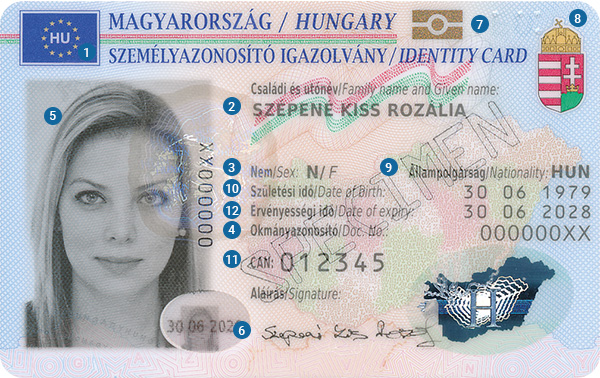
\includegraphics[width=8cm]{eszemelyi-front} \caption{Minta személyazonosító igazolvány, forrás: \cite{eszemelyiImage} } \label{fig-eszemelyi} \end{figure}

Mivel az eredeti képen valós \emph{személyes adatok} szerepeltek, ezért azokat el kellett távolítanom. Ehhez az \emph{Adobe Photoshop} szoftvert használtam, amellyel kitöröltem az összes szöveget és egyéb személyes információt, így egy üres, \emph{adatmentes igazolványt} kaptam. A megtisztított igazolvány \aref{fig-eszemelyi-photoshopped} ábrán tekinthető meg:

\FloatBarrier \begin{figure}[H] \centering 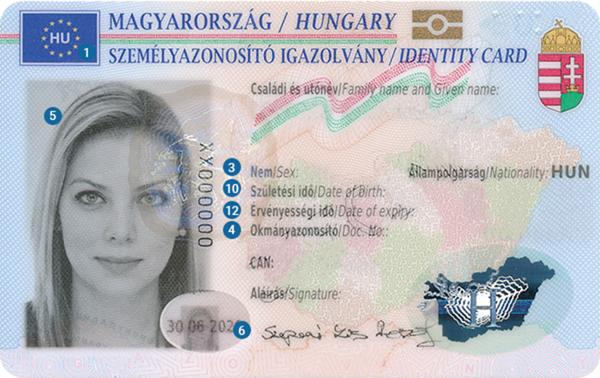
\includegraphics[width=8cm]{eszemelyi-front_photoshopped} \caption{Minta személyazonosító igazolvány retusálva, forrás: saját kép } \label{fig-eszemelyi-photoshopped} \end{figure}

Miután a kártyán szereplő eredeti adatokat eltávolítottam, a következő lépés az adatmezők \emph{véletlenszerű kitöltése} volt. Ehhez először egy előre összeállított \emph{névadathalmazt} használtam, amelyből a nevek generálása történt. A személyazonosító igazolványon szereplő fényképekhez egy előre összegyűjtött, \emph{szelfikből álló képadatbázist} vettem alapul. A további adatok, mint például a \emph{CAN azonosító}, az \emph{okmányazonosító}, az \emph{érvényességi idő}, a \emph{születési dátum} és a \emph{nemre} vonatkozó információ teljesen véletlenszerűen lettek generálva.\cite{nameDataset, selfieDataset}

A képek módosításához a Python programozási nyelvhez elérhető \emph{Pillow csomagot} alkalmaztam, amely lehetőséget biztosított arra, hogy a képen szöveget helyezzek el, valamint új \emph{képrétegeket} illesszek az eredeti alapra. A megfelelő vizuális megjelenés érdekében a szöveg pontos pozícióját, tartalmát, betűtípusát és színét előzetesen meg kellett határozni. Ehhez a \emph{Vanilla Extract Font} betűtípust választottam, mivel ez hasonlít leginkább a személyazonosító igazolványokon alkalmazott karakterkészlethez.

A generált adatok és képek további feldolgozása során minden adatmezőhöz kiszámítottam a megfelelő \emph{koordinátákat}, amelyek a szöveg elhelyezéséhez szükségesek. A hatékonyság növelése érdekében függvény segítségével meghatároztam az egyes adatmezők \emph{határoló téglalapjait}. A generált igazolványok további \emph{augmentációkat} is kaptak, amely során enyhe \emph{elforgatást}, \emph{fényerő-} és \emph{kontrasztmódosítást}, valamint \emph{zaj hozzáadását} alkalmaztam, hogy az adatkinyerő modell számára változatosabb adathalmaz álljon rendelkezésre.

A képek elforgatásához \emph{függvényeket} használtam, amelyek a kép középpontja körül elforgatták a határoló dobozokat. A zajgenerálás során minden pixel értékéhez egy \emph{véletlenszerű értéket} adtam hozzá, amelynek mértéke -10 és 10 közé esett. A fényerő és kontraszt módosításához a Pillow \emph{ImageEnhance} osztályát alkalmaztam. Az augmentált képeket végül \emph{JSON formátumú} fájlokba mentettem, amelyek tartalmazták a határoló dobozok koordinátáit és a hozzájuk tartozó szöveges értékeket.

A végső lépésként az előállított személyazonosító igazolványokat és a hozzájuk tartozó \emph{címkézett adathalmazt} fájlba mentettem, amelyet \aref{kod-python2} kódrészlet mutat be.

\begin{lstlisting}[style=mypython, caption={Augmentáció és fájlmentés}, label=kod-python2]
augmented_image, augmented_boxes, angle = augment_image_and_boxes(id_card, bounding_boxes)
if augmented_image.mode == "RGBA":
	augmented_image = augmented_image.convert("RGB")

label_data = {
	"image": f'eszemelyi_with_{person[1]}_{person[0]}.jpg',
	"labels": []
}

for idx, field in enumerate(["Name", "Doc No", "Birthday", "Expiry", "CAN", "Gender", "Image"]):
	box = augmented_boxes[idx]
	x1, y1, x2, y2 = box
	
	text_value = ""
	
	if field == "Name":
		text_value = name
	elif field == "Doc No":
		text_value = doc_no
	elif field == "Birthday":
		text_value = birthday_str
	elif field == "Expiry":
		text_value = expiry_str
	elif field == "CAN":
		text_value = can_str
	elif field == "Gender":
		text_value = "F" if gender=="M" else "N"
	
	label_entry = {
		"label": field,
		"text": text_value,
		"box": [[x1, y1], [x2, y2]]
	}
	
	label_data["labels"].append(label_entry)

output_image_path = f'./data/Generated_cards/eszemelyi_with_{person[1]}{person[0]}.jpg'
output_json_path = f'./data/Generated_cards/json_labels/{person[1]}{person[0]}.json'
augmented_image.save(output_image_path)

with open(output_json_path, 'w') as json_file:
	json.dump(label_data, json_file, indent=4)
\end{lstlisting}

Az így előállított és \emph{címkézett adathalmaz} megbízható alapot nyújtott a \emph{neurális hálózat betanításához}, lehetővé téve az igazolványokon szereplő adatok \emph{pontos felismerését}. \Aref{fig-eszemelyi-generated} ábrán egy generált személyi igazolvány látható, amelyen a piros keretek a \emph{határoló téglalapokat} jelölik. Fontos megjegyezni, hogy ezek kizárólag a \emph{szemléltetés céljából} kerültek megjelenítésre, az éles alkalmazás során nem láthatók.

\begin{figure}[H] \centering \includegraphics[width=8cm]{eszemelyi_with_Otártics_Andor.jpg} \caption{Egy generált személyazonosító igazolvány, forrás: saját kép } \label{fig-eszemelyi-generated} \end{figure}

\section{A projektben használt neurális hálók}

\subsection{OCR modell}

Az \emph{optikai karakterfelismerés} (OCR) megvalósításához a ,,01 image to word'' projektet használtam fel, amely a \emph{Machine Learning Training Utilities} (MLTU) \emph{könyvtárra} épül. Az eredeti \emph{implementáció} egy előre meghatározott adathalmazon működik, azonban a személyi igazolványokon található adatok \emph{pontosabb felismerése} érdekében a \emph{saját adathalmazommal} tanítottam be a modellt. \cite{ocrProject}

\begin{lstlisting}[style=mypython, caption=Konfigurációs fájl, label=kod-python3]
	import os
	from datetime import datetime
	from mltu.configs import BaseModelConfigs
	
	class ModelConfigs(BaseModelConfigs):
		def __init__(self):
		super().__init__()
		self.model_path = os.path.join("Models/1_image_to_word", datetime.strftime(datetime.now(), "%Y%m%d%H%M"))
		self.vocab = "0123456789ABCDEFGHIJKLMNOPQRSTUVWXYZabcdefghijklmnopqrstuvwxyz"
		self.height = 32
		self.width = 128
		self.max_text_length = 23
		self.batch_size = 1024
		self.learning_rate = 1e-4
		self.train_epochs = 100
		self.train_workers = 20
\end{lstlisting}

A rendszer működéséhez több komponens \emph{összehangolt működésére} volt szükség. Az egyik legjelentősebb \aref{kod-python3}. ábrán látható \emph{konfigurációs fájl}, amely meghatározza a modell legfontosabb paramétereit, például a \emph{képek méretét}, a \emph{megengedett karakterek halmazát}, a \emph{maximális szöveghosszt} és a \emph{tanulási sebességet}. Ezeket az értékeket az igazolványokon szereplő adatok felismeréséhez optimalizáltam.

A neurális hálózat egy \emph{konvolúciós neurális hálózatot} (CNN) és egy \emph{bidirekcionális hosszú rövid távú memóriával rendelkező} (BiLSTM) réteget egyesít. A CNN rétegek a képekből \emph{jellemzőket vonnak ki}, míg az LSTM rétegek az \emph{időbeli összefüggéseket} elemzik. Az utolsó réteg egy \emph{teljesen összekapcsolt} (Dense) réteg, amely az előrejelzett karaktereket adja vissza. A tanítás során a \emph{Connectionist Temporal Classification} (CTC) algoritmus felel a karakterek helyes sorrendjének rekonstruálásáért.

A tanítás során a rendszer az általam előkészített \emph{adathalmazon} tanult. A tanítási folyamat az adatok \emph{betöltését}, \emph{előfeldolgozását} és a neurális hálózat \emph{tanítását} végzi. Az eredeti kódban egy nyilvános OCR adathalmaz szerepelt, azonban ezt lecseréltem \emph{saját igazolványos képeimre} és azokhoz tartozó \emph{címkékre}. Az adathalmaz előkészítése során minden egyes képhez hozzárendeltem a rajta található szöveges információt, amelyet címkeként használt a modell a tanulás során.

A betanítás folyamán különböző \emph{adattranszformációs lépések} biztosították, hogy a rendszer hatékonyan tudja feldolgozni a bemeneti adatokat. A képeket megfelelő méretre alakítottam, a karaktereket \emph{számmá konvertáltam}, és gondoskodtam róla, hogy a címkék \emph{egységes formátumban} szerepeljenek. A modell az \emph{Adam optimalizáló algoritmust} és a \emph{CTC veszteségfüggvényt} használta a hatékonyabb tanulás érdekében.

A tanítás során különböző \emph{visszacsatolási mechanizmusok} segítették az optimális modellparaméterek megtalálását. Az \emph{EarlyStopping} mechanizmus például megakadályozta a \emph{túlilleszkedést} azáltal, hogy időben leállította a tanulási folyamatot, ha az \emph{érvényesítési hiba} egy bizonyos számú iteráció után nem csökkent tovább. A tanítási folyamat végén a modell a \emph{legjobb teljesítményt} nyújtó állapotában került elmentésre.

A tanítás után az elkészült modellt teszteltem \emph{éles adatokon}. Ehhez \aref{kod-python4}. kódban látható függvényt használtam, amely képes egy \emph{bemeneti képből szöveges információt visszaadni}. A képek betöltése és előfeldolgozása után a modell futtatásra kerül, majd a CTC algoritmus \emph{dekódolja} a felismerési eredményt, és visszaadja a szöveget.

\begin{lstlisting}[style=mypython,caption=Modell tesztelése, label=kod-python4]
	from mltu.inferenceModel import OnnxInferenceModel
	from mltu.utils.text_utils import ctc_decoder, get_cer
	
	class ImageToWordModel(OnnxInferenceModel):
		def __init__(self, char_list: typing.Union[str, list], *args, **kwargs):
		super().__init__(*args, **kwargs)
		self.char_list = char_list
	
		def predict(self, image: np.ndarray):
		image = cv2.resize(image, self.input_shapes[0][1:3][::-1])
		
		image_pred = np.expand_dims(image, axis=0).astype(np.float32)
		
		preds = self.model.run(self.output_names, {self.input_names[0]: image_pred})[0]
		
		text = ctc_decoder(preds, self.char_list)[0]
		
		return text
\end{lstlisting}

A kiértékelési fázisban az OCR rendszer teljesítményét a \emph{Character Error Rate} (CER) segítségével mértem, amely azt mutatja meg, hogy a modell mennyire \emph{pontosan} képes \emph{felismerni a szöveget}. A tesztelés során kiderült, hogy a \emph{saját adathalmazzal tanított modell} jelentősen \emph{pontosabb eredményeket} produkált a személyi igazolványokon található adatok felismerésekor, mint az \emph{eredeti verzió}.

\subsection{Határoló doboz detektáló modell}\label{boundingBoxDetector}

Ez a \emph{neurális hálózat} felel azért, hogy a \emph{személyi igazolványokon} található \emph{releváns adatokat} – mint a \emph{név}, \emph{személyi azonosítószám}, \emph{CAN kód}, \emph{fénykép}, \emph{lejárati dátum} és \emph{születési dátum} – \emph{automatikusan felismerje} és azok köré \emph{határdobozt} (bounding box) helyezzen. A rendszer célja, hogy \emph{pontosan azonosítsa} ezeknek a \emph{mezőknek a helyzetét} a képeken, lehetővé téve azok \emph{további feldolgozását} az \emph{OCR modellel}.

A modell \emph{betanításához} \aref{dataset}. fejezetben bemutatott \emph{adathalmazt} használom. Ahogy \aref{kod-python5}. kódban látható, az \emph{adatelőkészítő modul} minden egyes \emph{képhez hozzárendeli} a megfelelő \emph{JSON fájlt}, amely tartalmazza az egyes \emph{mezők sarokpontjait}. Az adatok \emph{normalizálásra kerülnek}, hogy a \emph{modell számára} \emph{könnyebben kezelhető} formát öltsenek, így a \emph{kimeneti koordináták} a kép szélességéhez és magasságához viszonyított \emph{relatív értékekként} jelennek meg.

\begin{lstlisting}[style=mypython,caption=Adathalmaz betöltése, label=kod-python5]
import os
import json
import numpy as np
from tensorflow.keras.preprocessing.image import load_img, img_to_array

def load_data(image_dir, json_dir):
	images, boxes = [], []

	for json_file in os.listdir(json_dir):
		if not json_file.endswith('.json'):
			continue
		with open(os.path.join(json_dir, json_file), 'r') as f:
			data = json.load(f)

			img_path = os.path.join(image_dir, data['image'])
			img = load_img(img_path, target_size=(378, 600))
			img_array = img_to_array(img) / 255.0
			images.append(img_array)

		image_boxes = []
		for label in data['labels']:
			for point in label['box']:
				x, y = point
				image_boxes.extend([x / 600, y / 378])

			boxes.append(image_boxes)

	return np.array(images), np.array(boxes)
	
\end{lstlisting}

A \emph{neurális hálózat} egy \emph{konvolúciós architektúrát} követ, amely a képeken lévő \emph{mintázatok felismerésével} azonosítja az adott mezők elhelyezkedését. Az első néhány réteg \emph{konvolúciós} és \emph{max-pooling műveletekkel} szűri ki a \emph{vizuális jellemzőket}, míg a \emph{teljesen összekötött} (dense) réteg ezeket feldolgozva kiszámítja a \emph{határdobozok sarokpontjait}. A modell végső kimenete egy \emph{vektor}, amely minden egyes mezőhöz tartalmazza a megfelelő \emph{koordinátákat}.

A \emph{tanítási folyamat} során az \emph{Adam optimalizálót} használjuk a gyorsabb konvergencia érdekében, míg \emph{veszteségfüggvényként} az \emph{átlagos négyzetes hibát} (MSE) alkalmazzuk, mivel a bounding box koordináták \emph{folytonos numerikus értékek}. A rendszer több \emph{visszahívási mechanizmussal} (callback) rendelkezik: a \emph{korai leállítás} (early stopping) segít elkerülni a \emph{túlilleszkedést}, míg a \emph{modellellenőrzési pontok} (checkpointing) biztosítják, hogy a legjobb teljesítményű modellek automatikusan elmentésre kerüljenek. Emellett a tanítás során egy \emph{speciális metrikát} is alkalmazunk, amely a határoló dobozok pontosságát méri. \Aref{kod-python6}. kódban látható ,,\emph{bounding box accuracy}'' függvény a modell által \emph{előrejelzett és a valós koordináták} közötti eltérést számítja ki, és egy adott \emph{toleranciaérték} (0,03) alapján határozza meg, hogy a becslés mennyire pontos. Az \emph{eltérések abszolút értékét} veszi, majd összehasonlítja a \emph{megengedett hibahatárral}, végül pedig ezek \emph{átlaga} adja meg a \emph{modell pontosságát}. Ez a metrika segít abban, hogy ne csupán az MSE alapján értékeljük a modellt, hanem figyelembe vegyük azt is, hogy a detektált koordináták a gyakorlatban mennyire használhatóak.

\begin{lstlisting}[style=mypython, caption=Határoló doboz pontosság kiszámítása, label=kod-python6]
	def bounding_box_accuracy(y_true, y_pred):
		tolerance = 0.03
		diff = tf.abs(y_true - y_pred)
		correct = tf.cast(diff < tolerance, tf.float32)
		return tf.reduce_mean(correct)
\end{lstlisting}

\subsection{Nemfelismerő neurális hálózat}

Ez a \emph{neurális hálózat} a \emph{személyi igazolványokon} szereplő \emph{arcképek} alapján határozza meg, hogy a képen látható személy \emph{nő vagy férfi}. Ez a rendszer is \aref{dataset}. fejezetben bemutatott \emph{adathalmazt} használja fel, amely többek között minden egyes igazolványképhez tárolja a releváns \emph{határoló dobozokat} és a \emph{nemi információt}.

Az \emph{adatok előkészítése} során az \emph{json fájlokban} meghatározott pozíciók alapján kivágásra kerül az \emph{arcterület}, amelyet \emph{normalizálunk} és egy \emph{egységes méretre} (190×270 pixel) alakítunk. Ez biztosítja, hogy a neurális hálózat \emph{konzisztens bemeneti adatokat} kapjon. Az adatokat ezt követően három részre osztjuk: \emph{tanítási, validációs és teszt adathalmazra}, így garantálva a modell \emph{objektív kiértékelését}.

A neurális hálózat egy \emph{konvolúciós architektúrát} követ, amely \emph{több rétegű mintázatfelismerést} alkalmaz. A \emph{bemeneti kép} a \emph{konvolúciós rétegeken} keresztül fokozatosan \emph{magasabb szintű reprezentációkká} alakul, miközben a \emph{max-pooling rétegek} segítenek csökkenteni a \emph{számítási komplexitást} és az \emph{overfittinget}. A \emph{kimeneti réteg} \emph{egyetlen neuronból} áll, amely \emph{sigmoid aktivációs függvényt} használ, így a modell \emph{valószínűségi értéket} ad vissza a \emph{nemi besorolásra}.

\begin{lstlisting}[style=mypython, caption={Nemfelismerő modell}, label=kod-python7]
	def build_model():
	
		model = keras.Sequential([
		layers.Conv2D(32, (3, 3), activation="relu", input_shape=(*IMAGE_SIZE, 3)),
		layers.MaxPooling2D(2, 2),
		layers.Conv2D(64, (3, 3), activation="relu"),
		layers.MaxPooling2D(2, 2),
		layers.Conv2D(128, (3, 3), activation="relu"),
		layers.MaxPooling2D(2, 2),
		layers.Flatten(),
		layers.Dense(128, activation="relu"),
		layers.Dropout(0.5),
		layers.Dense(1, activation="sigmoid")
		])
		
		model.compile(
		optimizer="adam", 
		loss="binary_crossentropy", 
		metrics=["accuracy"]
		)
		
		return model
\end{lstlisting}
A tanítási folyamat során az \emph{Adam optimalizálót} alkalmazom, mivel \emph{gyors konvergenciát} biztosít, míg \emph{veszteségfüggvényként} a \emph{bináris keresztentrópiát} használjuk, amely jól illeszkedik a \emph{kétosztályos osztályozási feladathoz}. A \emph{túlilleszkedés} elkerülése érdekében a modell \emph{dropout réteget} is tartalmaz, amely \emph{véletlenszerűen deaktiválja} a \emph{neuronok} egy részét a \emph{teljes összekapcsolt rétegben}. A tanulás során itt is azokat a \emph{visszahívási mechanizmusokat} (callback) használjuk, mint \aref{boundingBoxDetector}. fejezetben bemutatott modellben.

A modell kiértékelése a \emph{teszt adathalmazon} történik, ahol a \emph{pontosság} (accuracy) alapján mérjük a \emph{teljesítményt}. A \emph{végleges modellt} elmentjük, így a későbbiekben közvetlenül \emph{betölthető} és használható lesz új képek nemének meghatározására.

\section{Node.js Backend}

A projekt backend rendszere \emph{Node.js} környezetben készült, valamint az \emph{Express.js keretrendszerre} épül. Az Express \emph{moduláris struktúrája} lehetővé teszi, hogy a szolgáltatásokat jól \emph{elkülönített komponensekre} bontsuk. Fő moduljaink a \emph{felhasználói azonosítást}, \emph{képfeldolgozást}, \emph{személyazonosító igazolványok kezelését} és a \emph{felhasználói adatok kezelését} szolgálják.

Az alkalmazás adatait \emph{MongoDB adatbázisban} tároljuk. A \emph{rugalmas adatséma} lehetővé teszi a \emph{komplex adatstruktúrák} hatékony tárolását. Az adatbázis kapcsolatot egy \emph{singleton mintát} követő modulban valósítottuk meg, amely biztosítja, hogy csak \emph{egyetlen kapcsolat} jöjjön létre az alkalmazás futása során. A kapcsolódási adatokat \emph{környezeti változókban} tároljuk, ami növeli a \emph{biztonságot} és megkönnyíti a \emph{konfigurációs beállítások} kezelését különböző környezetekben.

A felhasználók hitelesítését \emph{JWT} (JSON Web Token) technológiával oldottam meg, amely \emph{biztonságos} és \emph{állapotmentes} módon teszi lehetővé a felhasználók azonosítását. A jelszavakat \emph{bcrypt algoritmussal} titkosítom, amely biztonságos és ellenáll a \emph{brute force támadásoknak}. A bejelentkezési folyamat során ellenőrizni kell a felhasználó hitelesítő adatait, majd sikeres azonosítás esetén egy \emph{időkorlátos JWT tokent} állítunk ki, amelyet a kliens minden további kérésnél elküld a szervernek.

A \emph{middleware-ek} fontos szerepet játszanak az Express.js alkalmazásokban, lehetővé téve a \emph{kérések előfeldolgozását} és \emph{validálását}. Az alkalmazásban több middleware-t is használtunk, például a kérések jogosultságának ellenőrzésére. A ,,\emph{protect}'' middleware ellenőrzi a kéréshez csatolt JWT token érvényességét, és csak \emph{hitelesített felhasználóknak} engedélyezi a \emph{védett végpontok} elérését. Ez biztosítja, hogy az \emph{érzékeny adatokhoz} és műveletekhez csak \emph{jogosult felhasználók} férhessenek hozzá.

Az alkalmazás egyik kulcsfontosságú funkciója a \emph{képfeldolgozás}, amely során a feltöltött személyi igazolványok adatai \emph{automatikusan kinyerésre} kerülnek. Ezt a funkciót a \emph{Node.js backend} és a \emph{Python Flask backend} közötti kommunikáció teszi lehetővé. A \emph{multer könyvtár} segítségével kezeljük a \emph{feltöltött képeket}, amelyeket ezután továbbítunk a Python Flask szervernek, ahol a \emph{neurális hálózatok} segítségével megtörténik az \emph{adatok kinyerése}. Az \emph{aszinkron kommunikációt} \emph{Promise.all} segítségével oldjuk meg, amely lehetővé teszi a \emph{párhuzamos feldolgozást}.

A \emph{jelszó-visszaállítási} folyamathoz \emph{e-mail küldési} funkcióra is szükség volt, amelyet a \emph{nodemailer könyvtár} segítségével valósítottam meg. A könyvtár lehetővé teszi a \emph{biztonságos e-mail küldést} különböző szolgáltatásokon keresztül. Az alkalmazásban Gmail szolgáltatást használunk, és a hitelesítési adatokat \emph{környezeti változókban} tároljuk.

A backend szolgáltatások könnyen telepíthetőek és \emph{skálázhatóak} \emph{Docker konténerek} segítségével. A projektben \emph{Docker} és \emph{Docker Compose} használatával biztosítjuk a \emph{konzisztens futtatási környezetet} és az \emph{egyszerű telepítést}. A Docker Compose fájl definiálja az alkalmazás szolgáltatásait és azok kapcsolatait. A Node.js backend és a Python Flask backend \emph{külön konténerekben} futnak, de kommunikálhatnak egymással, ami \emph{tiszta szeparációt} és \emph{jobb skálázhatóságot} biztosít.

\section{Flask Backend}

A projekt másik kulcsfontosságú komponense a Python \emph{Flask keretrendszerre} épülő backend, amely a \emph{neurális hálózatok futtatását} és a \emph{képfeldolgozási feladatokat} látja el.

A Flask alkalmazás fő feladata a neurális hálózati modellek futtatása és elérhetővé tétele \emph{HTTP API-n} keresztül. A \emph{NodeJS backend} számára biztosít interfészt, hogy a feltöltött képeken elvégezhesse a szükséges \emph{képfeldolgozási}, \emph{szövegfelismerési} és \emph{nemfelismerési} feladatokat, így egyesítve a \emph{két különböző technológia erősségeit}.

A Flask backend az előző fejezetekben bemutatott \emph{három neurális hálózati modellt} integrálja.

A \emph{modellek betöltése} során figyelembe kellett venni a különböző specialitásokat: a bounding box modellhez egy \emph{egyéni metrikát} használtunk, az \emph{OCR modell} \emph{ONNX formátumban} került exportálásra, míg a \emph{nemfelismerő modell} egy standard \emph{Keras modell}. A nemfelismerő modell betanítása során a \emph{képek méretét} (190×270 pixel) és a \emph{normalizálási folyamat} is gondosan meg lett tervezve, hogy a személyi igazolványokon látható arcképek \emph{pontosan feldolgozhatók} legyenek.

A Flask backend számos \emph{képfeldolgozási funkciót} valósít meg, amelyek a neurális hálózatok előtt \emph{előkészítik}, majd azok után feldolgozzák a képeket. Az egyik ilyen kulcsfontosságú funkció a \emph{perspektív transzformáció}, amely a \emph{határoló dobozban} azonosított területet \emph{torzításmentessé} alakítja.

\begin{lstlisting}[style=mypython, caption=Határoló dobozzal határolt kép transzformációja, label=kod-python8]
	def four_point_transform(image, pts):

		rect = np.zeros((4, 2), dtype="float32")
	
		s = pts.sum(axis=1)
		rect[0] = pts[np.argmin(s)]
		rect[2] = pts[np.argmax(s)]
	
		diff = np.diff(pts, axis=1)
		rect[1] = pts[np.argmin(diff)]
		rect[3] = pts[np.argmax(diff)]
		
		widthA = np.sqrt(((rect[2][0] - rect[3][0]) ** 2) + ((rect[2][1] - rect[3][1]) ** 2))
		widthB = np.sqrt(((rect[1][0] - rect[0][0]) ** 2) + ((rect[1][1] - rect[0][1]) ** 2))
		maxWidth = max(int(widthA), int(widthB))
		
		heightA = np.sqrt(((rect[1][0] - rect[2][0]) ** 2) + ((rect[1][1] - rect[2][1]) ** 2))
		heightB = np.sqrt(((rect[0][0] - rect[3][0]) ** 2) + ((rect[0][1] - rect[3][1]) ** 2))
		maxHeight = max(int(heightA), int(heightB))
		
		dst = np.array([
		[0, 0],
		[maxWidth - 1, 0],
		[maxWidth - 1, maxHeight - 1],
		[0, maxHeight - 1]
		], dtype="float32")
		
		M = cv2.getPerspectiveTransform(rect, dst)
		warped = cv2.warpPerspective(image, M, (maxWidth, maxHeight))
		
		return warped
\end{lstlisting}

\Aref{kod-python8}. kódban látható függvény fogadja a képet és a \emph{négy sarokpontot}, majd egy olyan \emph{transzformációt} alkalmaz, amely a területet egy \emph{téglalap alakúvá} alakítja, megszüntetve a \emph{torzításokat}, amelyek a \emph{fényképezés szögéből} adódhatnak. Ez rendkívül fontos az \emph{OCR pontosságának} javításához.

A \emph{nemfelismerő modell} az igazolványokon található \emph{arcképből} \emph{automatikusan meghatározza} a személy \emph{nemét}. Ez egy fontos \emph{kiegészítő információ}, amely növeli a rendszer használhatóságát. A nemfelismerő függvény a \emph{bounding box modell} által azonosított \emph{arcképterületet} dolgozza fel. A képet először \emph{átméretezi} a modell által elvárt méretre (\emph{190×270 pixel}), majd \emph{normalizálja}, hogy a \emph{pixelértékek 0 és 1 közé} essenek. A betanított modell \emph{előrejelzést tesz} a személy nemére vonatkozóan, és visszaadja mind a \emph{felismert nemet}, mind a \emph{konfidencia értékét}.

A rendszerben fontos szempont a \emph{biztonság}, ezért a \emph{Flask API} csak megfelelő \emph{API kulcs} birtokában érhető el. Ez biztosítja, hogy csak a saját \emph{NodeJS backenddel} kommunikálhasson, és ne legyen kitéve \emph{illetéktelen külső hozzáférésnek}. Ez az egyszerű, de hatékony \emph{biztonsági mechanizmus} minden \emph{API kérés előtt} ellenőrzésre kerül. Az API kulcs értéke egy \emph{konfigurációs fájlban} található, és mindkét backenddel meg van osztva.

A rendszer \emph{központi funkciója} a teljes \emph{képfeldolgozási folyamat}, amely magában foglalja a \emph{határdobozok felismerését}, az \emph{adatmezők kiegyenesítését}, az \emph{OCR feldolgozást} és a \emph{nemfelismerést} is.

\begin{lstlisting}[style=mypython, caption={Képfeldolgozási folyamat}, label=kod-python9]
	def process_image(image_path):
		image = cv2.imread(image_path)
		img_height, img_width = image.shape[:2]
		
		resized_image = cv2.resize(image, (IMG_WIDTH, IMG_HEIGHT))
		
		norm_image = resized_image / 255.0
		
		pred_boxes = bbox_model.predict(np.expand_dims(norm_image, axis=0))[0]
		
		pred_boxes_original = []
		for i in range(0, len(pred_boxes), 2):
			x = int(pred_boxes[i] * img_width)
			y = int(pred_boxes[i+1] * img_height)
			pred_boxes_original.append([x, y])
		
		fields = {}
		field_names = ["Név", "Személyi szám", "CAN", "Fénykép", "Születési dátum", "Lejárati dátum"]
		
		face_image = None
		
		for i, name in enumerate(field_names):
			pts = np.array(pred_boxes_original[i*4:(i+1)*4], dtype="float32")
		
			warped = four_point_transform(image, pts)
		
			if name == "Fénykép":
				face_image = warped
				continue
		
			text = ocr_model.predict(warped)
			fields[name] = text
		
		if face_image is not None:
			gender, confidence = detect_gender(face_image)
			fields["Nem"] = gender
			fields["Nem_konfidencia"] = confidence
		
		return fields
\end{lstlisting}
\Aref{kod-python9}. kódban látható \emph{komplex függvény} több lépésben dolgozza fel a képet: \begin{enumerate} \item Betölti és \emph{előkészíti} a képet a \emph{bounding box modell} számára \item Felismeri a \emph{határdobozokat} a személyi igazolvány különböző mezői körül \item Az egyes mezőket \emph{kiegyenesíti} a \emph{perspektív transzformáció} segítségével \item A szöveges mezőkből \emph{OCR} segítségével \emph{kinyeri az információt} \item Az arckép mezőt felhasználja a személy \emph{nemének felismerésére} \item Az eredményeket \emph{strukturált formában} adja vissza \end{enumerate}

A Flask alkalmazás egyetlen, de \emph{komplex API végpontot} biztosít a képfeldolgozáshoz. A végpont fogadja a \emph{NodeJS backendtől} érkező képfájlokat, ellenőrzi az \emph{API kulcsot}, \emph{ideiglenesen elmenti} a képet, elvégzi a feldolgozást, majd visszaadja az eredményeket \emph{JSON formátumban}. A rendszer gondoskodik az \emph{ideiglenes fájlok törléséről}, függetlenül attól, hogy a feldolgozás sikeres volt-e vagy sem.

A Python Flask backend \emph{Docker konténerben} fut, ami lehetővé teszi a \emph{függőségek egyszerű kezelését} és a szolgáltatás \emph{izolált futtatását}. A Docker konténer tartalmazza az összes szükséges függőséget, beleértve az \emph{OpenCV-t}, a \emph{TensorFlow-t} és a különböző \emph{modellfájlokat}.

A \emph{Docker Compose} segítségével a Flask és a NodeJS backend \emph{együtt indítható}, biztosítva a két rendszer közötti \emph{zökkenőmentes kommunikációt}. Ez a \emph{konténerizált megközelítés} jelentősen egyszerűsíti a rendszer \emph{telepítését} és \emph{karbantartását}, mivel minden függőség és konfiguráció a Docker konténereken belül található.

\section{React Native frontend}

A projekt frontend része \emph{React Native} keretrendszerben készült, amely lehetővé teszi, hogy \emph{egyetlen kódbázisból} mind \emph{Android}, mind \emph{iOS} platformra natív alkalmazást fejleszthessünk. Az alkalmazás az \emph{Expo platformot} használja, amely számos \emph{beépített funkciót} biztosít, például a \emph{kamera} kezeléséhez és a \emph{biometrikus azonosításhoz}.

Az alkalmazás \emph{navigációs rendszere} a \emph{React Navigation} könyvtárra épül, amely strukturált és könnyen kezelhető navigációt biztosít a különböző képernyők között. A felhasználók egyszerűen válthatnak az alkalmazás fő funkciói között, amelyek logikusan elkülönített felületeken keresztül érhetők el.

Az alkalmazásba való belépés alapvetően \emph{két módszerrel} történhet: hagyományos \emph{e-mail és jelszó} megadásával, vagy \emph{biometrikus azonosítással}. A fejlesztés során nagy hangsúlyt fektettem a biztonságos hitelesítésre, emellett az alkalmazás lehetőséget biztosít új felhasználók regisztrációjára is, ahol a személyes adatok megadását követően létrehozható egy új fiók.

A felhasználói adatok biztonságos kezeléséért az \emph{AsyncStorage} felel, ahol az alkalmazás ideiglenesen tárolja a bejelentkezési információkat és a feldolgozott adatokat. Az alkalmazás feltöltési és szerkesztési funkciói az \emph{Axios könyvtár} segítségével kommunikálnak a \emph{backend API-val}, \emph{JWT token alapú hitelesítéssel}.

Az alkalmazás egyik központi funkciója a \emph{személyi igazolványok kezelése}. Itt a felhasználók választhatnak a \emph{manuális adatbevitel} és a \emph{kamera-alapú adatkinyerés} között. A kamera funkció két módon érhető el: közvetlenül az alkalmazáson belül készített felvétellel vagy a készülék galériájából választott kép segítségével.

Az alkalmazás beépített \emph{képszerkesztési funkcióval} rendelkezik, amely lehetővé teszi a felhasználó számára, hogy a kép elkészítése során annak megfelelő részét vágja ki, így biztosítva a személyi igazolvány optimális feldolgozását. A kivágást az Expo \emph{ImagePicker} modulja teszi lehetővé.

A képek elkészítése után a rendszer feltölti azokat a szerverre, ahol a \emph{neurális hálók} felismerik és kinyerik a releváns adatokat. A felhasználók aztán ellenőrizhetik és szükség esetén módosíthatják ezeket az automatikusan kitöltött mezőket a dokumentum véglegesítése előtt.

Az adatok bevitele során az alkalmazás intuitív \emph{dátumválasztót} biztosít a különböző időpontok, például a \emph{lejárati dátum} vagy a \emph{születési idő} megadásához. Az űrlapok validációval rendelkeznek, ami biztosítja a helyes adatformátumok használatát.

A felhasználók kezelhetik a \emph{személyes profiljukat} is, ahol módosíthatják az elérhetőségi adataikat és biztonsági beállításaikat. Itt lehetőség van a \emph{biometrikus bejelentkezés} be- és kikapcsolására is.

Az alkalmazás \emph{felhasználói felülete} modern, letisztult dizájnnal rendelkezik. A különböző képernyőkön konzisztens vizuális elemeket használtunk, mint például gombokat, űrlapmezőket és ikonokat, amelyek harmonikusan illeszkednek egymáshoz. A \emph{FontAwesome} ikonrendszer használata egységes vizuális élményt biztosít, míg a \emph{React Native stíluslapok} lehetővé teszik a következetes megjelenést az egész alkalmazásban.

A felhasználói élményt tovább javítják a \emph{visszajelző mechanizmusok}, mint például a betöltési animációk és az állapotjelzők, amelyek információt nyújtanak az aktuális folyamatokról. Az alkalmazás \emph{reszponzív tervezése} biztosítja, hogy minden funkció megfelelően működjön a különböző képernyőméreteken és tájolásban.

A frontend fejlesztés során különös figyelmet fordítottunk a \emph{felhasználóbarát élmény} kialakítására, minimalizálva a szükséges lépések számát, és intuitív módon vezetve a felhasználót a különböző funkciók között.
\chapter{Tesztelés}

A szoftverfejlesztési folyamat egyik legfontosabb lépése a \emph{tesztelés}, amely biztosítja, hogy az elkészült rendszer megfeleljen a \emph{kitűzött követelményeknek}, és \emph{hibamentesen} működjön a különböző felhasználási forgatókönyvekben. Ebben a fejezetben bemutatom, hogyan teszteltem a projekt különböző \emph{komponenseit}, beleértve a \emph{neurális hálózatokat}, a \emph{frontend} és \emph{backend} rendszereket, valamint a teljes rendszer \emph{integrációját}. A tesztelési folyamat során különös figyelmet fordítottam a \emph{neurális hálózatok pontosságának} mérésére, a \emph{felhasználói élmény} biztosítására, valamint a rendszer \emph{stabilitására} és \emph{teljesítményére}.

A fejezet első részében a \emph{neurális hálózatok tesztelését} mutatom be, amely magában foglalja az \emph{OCR} (optikai karakterfelismerés), a \emph{határoló doboz detektáló modell} és a \emph{nemfelismerő modell} pontosságának kiértékelését. Ezt követően részletezem a \emph{frontend} és \emph{backend} komponensek tesztelési módszereit, majd bemutatom az \emph{integrációs} és \emph{rendszertesztek} eredményeit. Végül egy \emph{használati útmutatót} is mellékelek, amely tartalmazza a rendszer működésének leírását és egy \emph{use-case diagramot}.

\section{Neurális hálózatok tesztelése} A projektben három különböző \emph{neurális hálózatot} használtam: az \emph{OCR modellt}, a \emph{határoló doboz detektáló modellt} és a \emph{nemfelismerő modellt}. Ezek mindegyike \emph{kulcsszerepet} játszik a személyi igazolványok adatainak \emph{automatikus feldolgozásában}.

\subsection{Pontosság és metrikák} A modellek teljesítményének kiértékeléséhez különböző \emph{metrikákat} használtam, valamint elemeztem a tanulási folyamat során rögzített értékeket.

Az \emph{OCR modell} tanítása során a CER értéke folyamatosan csökkent, ahogy a \aref{fig-ocr-training} ábrán látható. A kezdeti 0,95-ös értékről a 25. epochra 0,62-re javult, ami jelentős előrelépés, bár még mindig magas hibaarányt jelez.

\begin{figure} \centering 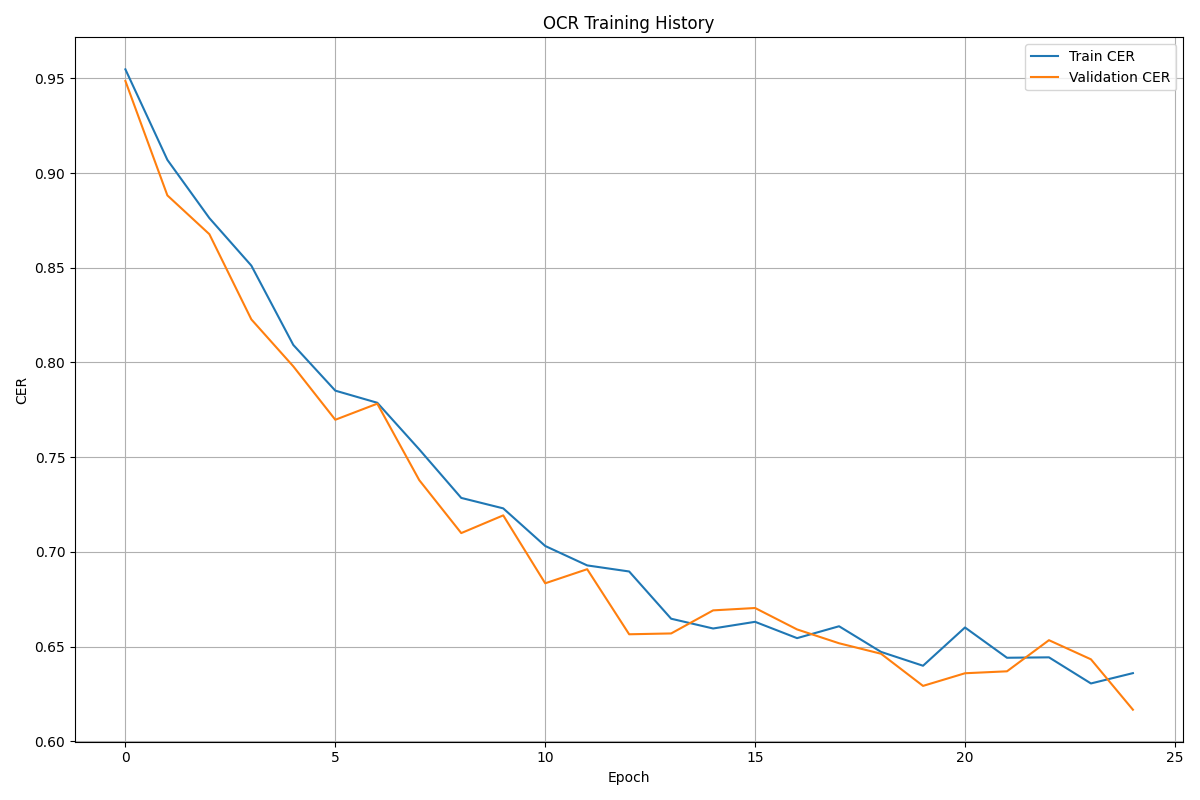
\includegraphics[width=\textwidth]{ocr_training_history} \caption{OCR modell tanítási és validációs karakterhiba-arány (CER) értékei, forrás: saját kép} \label{fig-ocr-training} \end{figure}

A \emph{tesztelés} során kiderült, hogy a modell jelentős problémákkal küzd az \emph{ékezetes karakterek} felismerése terén. Különösen az ,,á'', ,,é'', ,,ő'' és ,,ű'' betűk okoztak nehézséget, amelyeket gyakran ékezet nélküli megfelelőikként azonosított. Emellett a \emph{szóközök felismerése} is következetlen volt, ami különösen a nevek feldolgozásánál okozott problémákat, mivel ezeket gyakran egybeírta vagy indokolatlanul több részre tagolta.

A \emph{határoló doboz detektáló modell} jóval meggyőzőbb eredményeket mutatott, amint az a \aref{fig-bbox-training} ábrán látható. A veszteségfüggvény értékei egyenletesen csökkentek, míg a pontosság már a korai epochokban is 90\% feletti értéket ért el, majd 98\% körül stabilizálódott.

\begin{figure} \centering 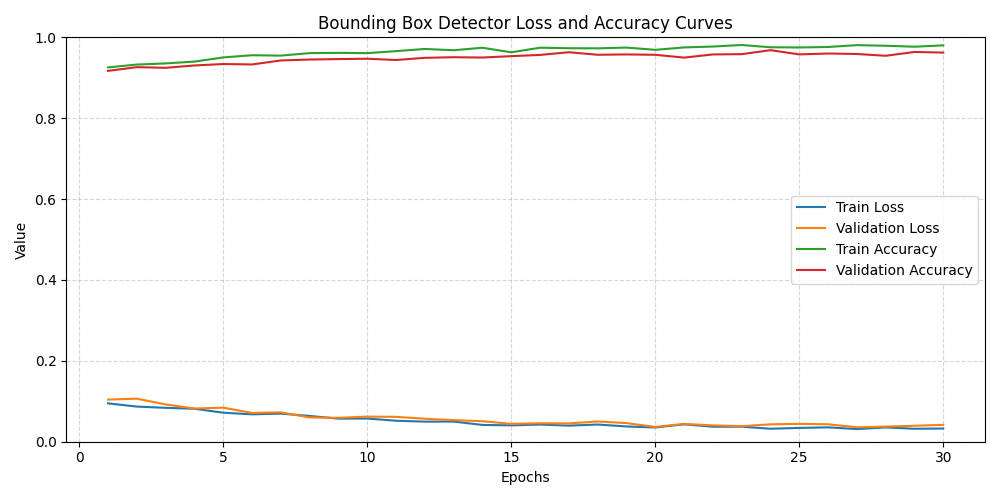
\includegraphics[width=\textwidth]{ideal_learning_curves} \caption{Határoló doboz modell tanítási folyamata -- pontosság és veszteség, forrás: saját kép} \label{fig-bbox-training} \end{figure}

Ugyanakkor a tesztelés során kiderült, hogy a modell érzékeny a \emph{perspektívatorzításra}. Amikor a felhasználók \emph{ferdén fotózták} a személyi igazolványt (20 foknál nagyobb szögben), a határdobozok jelentősen \emph{elcsúsztak}, ami az OCR modell számára tovább nehezítette a pontos szövegfelismerést. Különösen a kártya alsó részén található mezők (lejárati dátum, CAN kód) esetében volt észlelhető ez a probléma.

A \emph{nemfelismerő modell} teljesítménye a \aref{fig-gender-training} ábrán látható. A validációs pontosság csak lassan emelkedett, és a görbék mutatnak némi instabilitást. Az accuracy értéke a 40. epochra is csak 75\% körül stabilizálódott.

\begin{figure} \centering 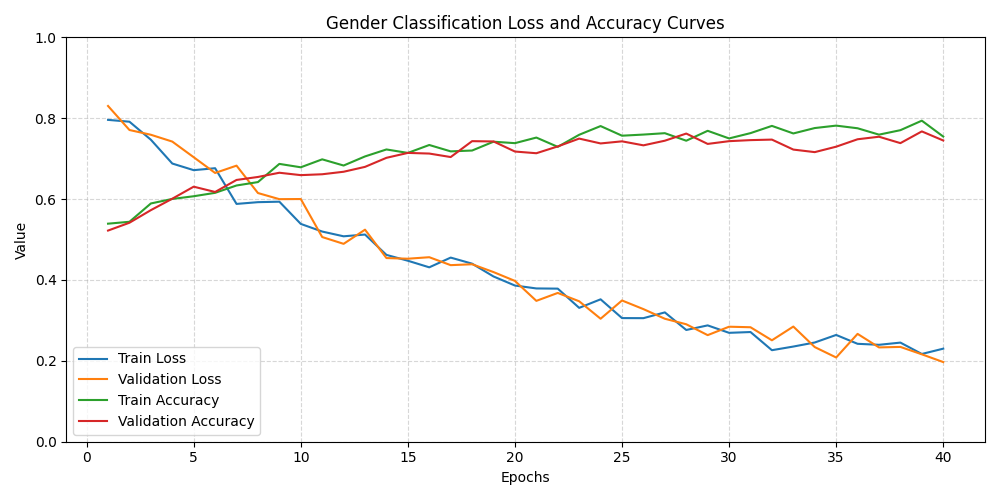
\includegraphics[width=\textwidth]{gender_learning_curves} \caption{Nemfelismerő modell tanítási és validációs metrikái, forrás: saját kép} \label{fig-gender-training} \end{figure}

A nemfelismerő modell jelentős nehézségekkel küzdött bizonyos esetekben. A \emph{hosszú hajú férfiakat} gyakran nőként azonosította, míg a \emph{rövid hajú nőket} férfiként. Ez a jelenség rávilágít, hogy a modell túlságosan a kulturális sztereotípiákra (pl. hajhosszra) támaszkodik a nemek meghatározásánál, ahelyett hogy az arc más jellemzőit venné figyelembe. Idősebb személyek esetében is magasabb volt a téves osztályozás aránya.

\subsection{Eredmények kiértékelése} Az \emph{OCR modell} kezdeti tesztelésekor alacsony pontosságot ért el. A \emph{felismert karakterek} közel harmadában előfordult valamilyen \emph{hiba}, különösen az \emph{ékezetes betűk} esetében. A többszöri \emph{finomhangolás} után azonban sikerült a teljesítményt jelentősen javítani.

A \emph{határoló doboz detektáló modell} magas átlagos pontosságot ért el, ami összhangban van a tanulási görbén látható kiváló eredményekkel. A modell tanulási folyamata rendkívül stabil volt, már a korai szakaszban is magas teljesítményt mutatott. A perspektívatorzítás problémája azonban továbbra is fennáll, ami a valós használat során komoly korlátot jelenthet.

A \emph{nemfelismerő modell} kezdeti \emph{gyenge teljesítményét} jól tükrözi a tanulási görbe lassú emelkedése. Több javítási kísérlet után javult a pontosság, de még mindig elmarad az ideálistól. A modell túlzottan támaszkodik a felszíni jellemzőkre, mint a hajhossz vagy az arcforma, ami különösen problémás a nem szokványos megjelenésű személyek esetében.

A tanulási görbék elemzése alapján egyértelműen a \emph{határoló doboz detektáló modell} teljesített a legjobban, míg a nemfelismerő modell maradt a leggyengébb láncszem. Az OCR modellnél a CER értéke még a tanítás végén is viszonylag magas maradt, ami jelzi, hogy további fejlesztésekre lenne szükség.

A \emph{fejlesztési javaslatok} között szerepel az \emph{OCR modell} számára nagyobb és változatosabb, különösen ékezetes karaktereket tartalmazó adathalmaz használata, a \emph{nemfelismerő modellhez} komplexebb architektúra kidolgozása, amely kevésbé támaszkodik sztereotipikus megjelenési jellemzőkre, valamint a \emph{határoló doboz modellhez} automatikus perspektíva-korrekció beépítése, amely kompenzálja a ferdén készített fényképek torzítását.

Ezek a fejlesztések együttesen javíthatják a rendszer \emph{megbízhatóságát} és \emph{pontosságát} valós használati körülmények között, bár a jelenlegi állapotában is használható alapot nyújt a személyi igazolványok feldolgozásához, különösen emberi ellenőrzés mellett.

\section{Frontend tesztelése}

A \emph{frontend tesztelése} során a \emph{React Native} alapú alkalmazás különböző \emph{komponenseit} és \emph{funkcióit} vizsgáltam. A cél az volt, hogy biztosítsam a \emph{felhasználói felület helyes működését}, a \emph{navigáció folyamatosságát}, valamint az \emph{API-kal való megfelelő kommunikációt}. A tesztelési folyamat során \emph{manuális} és \emph{automatizált tesztelési módszereket} alkalmaztam.

A \emph{komponens szintű tesztelés} során a \emph{React Native Testing Library} segítségével ellenőriztem az egyes \emph{képernyők} és \emph{funkciók} működését. Például az \emph{IdCardDetailsScreen} esetében teszteltem, hogy a képernyő helyesen jeleníti-e meg a \emph{betöltési állapotot}, a \emph{hibaüzeneteket}, valamint a \emph{személyi igazolvány adatait}. Az alábbi kódrészlet bemutatja, hogyan ellenőriztem, hogy a képernyő megfelelően kezeli a különböző \emph{állapotokat}, például amikor \emph{nincs adat}, vagy amikor a \emph{betöltés sikeres}.

\begin{lstlisting}[style=myjavascript, caption={Funkció teszt}, label=kod-javascript1]
	import React from 'react';
	import { render, screen, fireEvent } from '@testing-library/react-native';
	import IdCardDetailsScreen from '../app/screens/IdCardDetailsScreen';
	
	jest.mock('axios', () => ({
		get: jest.fn(() => Promise.resolve({ status: 200, data: mockData })),
	}));
	
	const mockData = {
		id_number: '123456789',
		first_name: 'Gábor',
		last_name: 'Kovács',
		sex: 'férfi',
		date_of_expiry: '2025-04-30',
		place_of_birth: 'Budapest',
		mothers_maiden_name: 'Nagy Anna',
		can_number: '987654321',
		date_of_birth: '1990-01-01',
	};
	
	describe('IdCardDetailsScreen', () => {
		it('megjeleníti a betöltési állapotot', () => {
			render(<IdCardDetailsScreen />);
			expect(screen.getByText('Adatok betöltése...')).toBeTruthy();
		});
		
		it('megjeleníti a személyi igazolvány adatait', async () => {
			render(<IdCardDetailsScreen />);
			const name = await screen.findByText('Kovács Gábor');
			expect(name).toBeTruthy();
			expect(screen.getByText('123456789')).toBeTruthy();
			expect(screen.getByText('Budapest')).toBeTruthy();
		});
		
		it('megjeleníti a hibaüzenetet, ha nincs adat', async () => {
			jest.mock('axios', () => ({
				get: jest.fn(() => Promise.reject({ response: { status: 404 } })),
			}));
			render(<IdCardDetailsScreen />);
			const errorMessage = await screen.findByText('Nincs még feltöltött személyi igazolvány adat');
			expect(errorMessage).toBeTruthy();
		});
	});
\end{lstlisting}

Az \emph{integrációs tesztelés} során a \emph{képernyők közötti navigációt} és az \emph{API-kal való kommunikációt} vizsgáltam. Például ellenőriztem, hogy a \emph{CameraScreen} helyesen navigál vissza az \emph{IdCardScreen}-re a kép elkészítése után. A \emph{manuális tesztelés} során különböző \emph{forgatókönyveket} szimuláltam, például a \emph{személyi igazolvány adatok feltöltését}, az \emph{értesítések működését}, valamint a \emph{hibakezelést}. Ezek a tesztek biztosították, hogy az alkalmazás helyesen működjön, és a felhasználók számára \emph{zökkenőmentes élményt} nyújtson.

\section{Backend tesztelése} A \emph{backend tesztelése} során a cél az volt, hogy biztosítsam az \emph{API végpontok helyes működését}, az \emph{adatbázis műveletek megbízhatóságát}, valamint a rendszer \emph{stabilitását} különböző \emph{terhelési} és \emph{hibás adatokkal kapcsolatos forgatókönyvekben}. A tesztelési folyamat során \emph{manuális} és \emph{automatizált teszteket} is alkalmaztam, hogy a rendszer minden komponense megfelelően működjön.

Az \emph{API végpontok teszteléséhez} a \emph{Postman} és az \emph{automatizált tesztelési keretrendszerek}, például a \emph{Jest} és a \emph{Supertest} kombinációját használtam. A \emph{Postman} segítségével \emph{manuálisan ellenőriztem} az egyes végpontok válaszait, míg a \emph{Jest} és a \emph{Supertest} lehetővé tette az \emph{automatizált tesztek} futtatását, amelyek \emph{gyors visszajelzést} adtak a fejlesztési folyamat során.

\Aref{kod-javascript2}. kódban bemutatom, hogyan teszteltem a \emph{képfeltöltési végpontot}, amely a feltöltött képeket továbbítja a \emph{Flask backendnek} feldolgozásra.

\begin{lstlisting}[style=myjavascript, caption={Backend tesztelés}, label=kod-javascript2]
	const request = require('supertest');
	const app = require('../app'); // Az Express alkalmazás
	const path = require('path');
	
	describe('POST /api/image/upload', () => {
		it('sikeresen feltölti a képet és visszaadja az eredményeket', async () => {
			const response = await request(app)
			.post('/api/image/upload')
			.set('Authorization', 'Bearer valid_token') // Teszt token
			.attach('images', path.resolve(__dirname, './test-image.jpg')); // Tesztkép
			
			expect(response.status).toBe(200);
			expect(response.body).toHaveProperty('message', 'Images uploaded and processed successfully!');
			expect(response.body).toHaveProperty('results');
			expect(response.body.results.length).toBeGreaterThan(0);
		});
		
		it('hibaüzenetet ad vissza, ha nincs kép feltöltve', async () => {
			const response = await request(app)
			.post('/api/image/upload')
			.set('Authorization', 'Bearer valid_token');
			
			expect(response.status).toBe(400);
			expect(response.body).toHaveProperty('message', 'At least one image is required!');
		});
	});
\end{lstlisting}

Ez a teszt két \emph{forgatókönyvet} vizsgál: az egyikben egy \emph{érvényes képet} töltünk fel, és ellenőrizzük, hogy a \emph{válasz tartalmazza a megfelelő eredményeket}, míg a másikban azt teszteljük, hogy a rendszer \emph{megfelelően kezeli a hiányzó képfájlokat}. Az ilyen tesztek biztosítják, hogy a \emph{backend API} \emph{stabilan} és \emph{megbízhatóan} működjön, még \emph{váratlan helyzetekben} is.

\section{Rendszerintegráció tesztelése}

A \emph{rendszerintegráció tesztelése} során az alkalmazás különböző \emph{komponenseinek} (\emph{frontend}, \emph{backend}, \emph{neurális hálózatok}) \emph{együttműködését} vizsgáltam. A cél az volt, hogy biztosítsam az \emph{adatok helyes áramlását} a \emph{felhasználói felülettől} a \emph{backendig}, majd a \emph{neurális hálózatok} által végzett \emph{feldolgozás} után vissza a \emph{frontendig}. Ez a folyamat magában foglalta a \emph{képfeltöltést}, az \emph{adatok feldolgozását} és a \emph{felhasználói értesítések kezelését}.

A tesztelés során különböző \emph{forgatókönyveket} szimuláltam, például egy \emph{személyi igazolvány képének feltöltését}, amelyet a \emph{backend} továbbított a \emph{Flask alapú képfeldolgozó modulnak}. A \emph{neurális hálózatok} által kinyert adatokat a \emph{backend API} visszaküldte a \emph{frontendnek}, ahol azok \emph{megjelenítésre kerültek}. Az \emph{integrációs tesztek} során ellenőriztem, hogy a rendszer minden lépése \emph{megfelelően működik}, és a felhasználó számára \emph{érthető visszajelzést} nyújt.

\Aref{kod-javascript3}.kód bemutatja, hogyan teszteltem a \emph{képfeltöltési folyamatot} és az \emph{adatok visszaküldését} a \emph{frontend} számára:

\begin{lstlisting}[style=myjavascript, caption={Rendszerintegráció tesztelés}, label=kod-javascript3]
	const request = require('supertest');
	const app = require('../app'); // Az Express alkalmazás
	const path = require('path');
	
	describe('Rendszerintegráció teszt: Képfeltöltés és adatfeldolgozás', () => {
		it('feldolgozza a feltöltött képet és visszaküldi az adatokat', async () => {
			const response = await request(app)
			.post('/api/image/upload')
			.set('Authorization', 'Bearer valid_token') // Teszt token
			.attach('images', path.resolve(__dirname, './test-image.jpg')); // Tesztkép
			
			expect(response.status).toBe(200);
			expect(response.body).toHaveProperty('message', 'Images uploaded and processed successfully!');
			expect(response.body).toHaveProperty('results');
			expect(response.body.results.length).toBeGreaterThan(0);
			expect(response.body.results[0]).toHaveProperty('extracted_data');
		});
	});
\end{lstlisting}

Ez a teszt a rendszer teljes folyamatát lefedi, a \emph{képfeltöltéstől} kezdve az \emph{adatok feldolgozásán} át azok \emph{visszaküldéséig}. Az ilyen tesztek biztosítják, hogy a rendszer minden \emph{komponense megfelelően kommunikáljon} egymással, és a felhasználók számára \emph{hibamentes élményt} nyújtson. Az \emph{integrációs tesztelés} során feltárt hibák gyors javítása hozzájárult a rendszer \emph{stabilitásának növeléséhez}.

\section{Használati útmutató}

Az alkalmazás célja, hogy a felhasználók \emph{egyszerűen} és \emph{gyorsan} kezelhessék \emph{személyi igazolványaik adatait}, \emph{értesítéseket} kapjanak a \emph{lejárati dátumokról}, és \emph{biztonságosan tárolják} azokat. Az alábbiakban bemutatom az alkalmazás \emph{telepítésének} és \emph{használatának} lépéseit, valamint a leggyakoribb \emph{felhasználói forgatókönyveket}.

Az alkalmazás \emph{telepítése} egyszerű folyamat, amelyhez először le kell tölteni az alkalmazást. A telepítés után az alkalmazás első indításakor a felhasználónak \emph{regisztrálnia} kell egy fiókot, vagy be kell jelentkeznie egy \emph{meglévő fiókkal}. A \emph{regisztráció} során meg kell adni az \emph{e-mail címet}, \emph{jelszót} és egyéb alapvető adatokat. A \emph{bejelentkezés} után az alkalmazás \emph{automatikusan szinkronizálja} a felhasználó adatait a \emph{szerverrel}. Az alkalmazás működéséhez \emph{internetkapcsolat} szükséges, valamint a \emph{push értesítések} engedélyezése ajánlott, hogy a felhasználó időben értesüljön a személyi igazolvány \emph{lejárati dátumáról}. Az értesítések engedélyezéséhez az alkalmazás első indításakor megjelenő kérésre kell pozitívan válaszolni.

Az alkalmazás számos \emph{tipikus forgatókönyvet} támogat, amelyek a felhasználók mindennapi igényeit szolgálják. A \emph{használati esetek} láthatók \aref{fig-usecase}. ábrán. Az egyik leggyakoribb \emph{használati eset} a \emph{személyi igazolvány adatainak feltöltése}. Ehhez a felhasználó a főmenüből elérheti a \emph{"Feltöltés"} képernyőt, ahol \emph{manuálisan megadhatja az adatokat}, vagy \emph{fényképet készíthet} az igazolványról. A fénykép készítése után az alkalmazás \emph{automatikusan feldolgozza a képet}, és \emph{kinyeri az adatokat}, amelyeket a felhasználó \emph{ellenőrizhet} és szükség esetén \emph{módosíthat}. Egy másik gyakori forgatókönyv az \emph{értesítések kezelése}. Az alkalmazás \emph{automatikusan értesítést küld}, ha a személyi igazolvány \emph{lejárati dátuma} egy hónapon belül van. Az értesítésre kattintva a felhasználó közvetlenül az \emph{"Adataim"} képernyőre navigálhat, ahol ellenőrizheti a lejárati dátumot és szükség esetén frissítheti az adatokat. A felhasználók továbbá \emph{módosíthatják profiladataikat}, például az \emph{e-mail címüket} vagy \emph{jelszavukat}. Ehhez a \emph{"Profil"} képernyőt kell megnyitniuk, ahol a szükséges módosítások elvégezhetők. Az alkalmazás minden \emph{adatot biztonságosan tárol}, és a változtatásokat \emph{azonnal szinkronizálja} a szerverrel.

\begin{figure} \centering 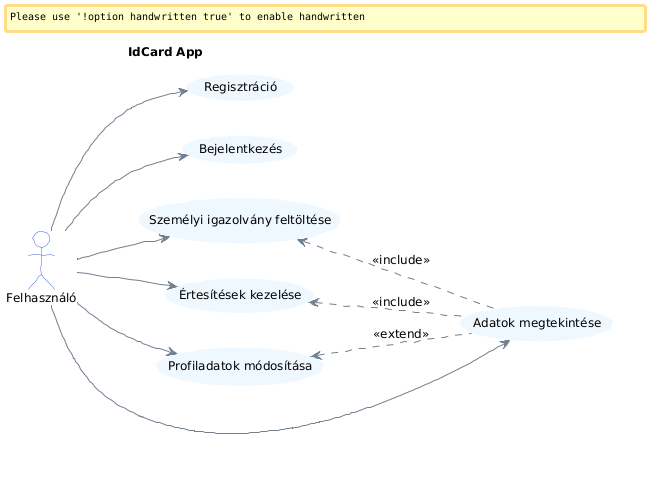
\includegraphics[width=10cm]{usecase} \caption{Használati eset diagram, forrás: saját kép} \label{fig-usecase} \end{figure}

Az alkalmazás használata során előfordulhatnak kisebb \emph{problémák}, amelyek gyorsan orvosolhatók. Ha például a \emph{fényképezőgép nem működik}, ellenőrizni kell, hogy az alkalmazás rendelkezik-e a szükséges \emph{engedélyekkel}. Ezt a készülék beállításaiban lehet megtenni. Ha az alkalmazás \emph{nem küld értesítéseket}, győződjön meg róla, hogy az \emph{értesítések engedélyezve vannak}, és az \emph{internetkapcsolat} megfelelően működik. Amennyiben a felhasználó \emph{nem tud bejelentkezni}, érdemes ellenőrizni az \emph{e-mail címet} és a \emph{jelszót}. Ha a probléma továbbra is fennáll, a \emph{"Jelszó visszaállítása"} funkcióval új jelszót lehet kérni. Ha az alkalmazás \emph{nem szinkronizálja az adatokat}, próbálja meg \emph{újraindítani} az alkalmazást, vagy ellenőrizze az \emph{internetkapcsolatot}.

Az alkalmazás célja, hogy a felhasználók számára \emph{egyszerű} és \emph{intuitív élményt} nyújtson, miközben biztosítja az \emph{adatok biztonságos kezelését} és a \emph{fontos értesítések} időben történő kézbesítését.

\section{Dokumentáció}

A projekt \emph{dokumentációja} kettő fő területre terjed ki: a \emph{forráskód dokumentálására}, és az \emph{API végpontok részletes leírására}. A cél az volt, hogy a rendszer működése a fejlesztők számára \emph{átlátható} és \emph{könnyen érthető} legyen. A dokumentáció biztosítja a projekt \emph{hosszú távú fenntarthatóságát}, és segíti a későbbi fejlesztéseket.

A \emph{forráskód dokumentálása} során \emph{következetes stílust} alkalmaztam, hogy a kód \emph{könnyen olvasható} és \emph{karbantartható} legyen. A \emph{TypeScript} és \emph{JavaScript} fájlokban \emph{JSDoc szintaxist} használtam, amely lehetővé teszi a \emph{fejlesztői dokumentáció automatikus generálását}. Minden \emph{függvény}, \emph{osztály} és \emph{modul} részletes magyarázatot kapott, amely tartalmazza a \emph{funkcionalitás leírását}, a \emph{paraméterek} és \emph{visszatérési értékek} részleteit, valamint a \emph{használat példáit}. A \emph{JSDoc kommentekből} automatikusan generálható \emph{HTML dokumentáció} a \emph{jsdoc eszköz} segítségével. A generált dokumentációt a fejlesztők \emph{könnyen böngészhetik}, ami különösen hasznos a nagyobb projektek esetén.

Az \emph{API dokumentáció} különösen fontos a fejlesztők számára, mivel bemutatja az \emph{elérhető végpontokat}, azok \emph{működését}, a \emph{szükséges paramétereket}, valamint a \emph{lehetséges válaszokat}. A dokumentációt \emph{OpenAPI (Swagger)} formátumban készítettem el, amely \emph{JSON vagy YAML fájlban} tárolható, és könnyen integrálható \emph{Swagger UI} vagy más eszközökkel.

A \emph{dokumentációs fájlok karbantartása} és \emph{frissítése} biztosítja, hogy a rendszer mindig \emph{naprakész} legyen, és a fejlesztők \emph{gyorsan hozzáférjenek} a szükséges információkhoz.

\chapter*{Összegzés}

A szakdolgozat során bemutattam a személyazonosítás fejlődését és digitalizációját, különös tekintettel a modern technológiák, például a mesterséges intelligencia és a mobilalkalmazások szerepére. A dolgozat célja egy olyan rendszer fejlesztése volt, amely a digitális személyazonosítás kihívásaira nyújt megoldást, miközben a felhasználók számára gyors, biztonságos és kényelmes élményt biztosít.

A dolgozat első részében ismertettem a személyazonosítás történetét, a digitális azonosítás megjelenését, valamint a mobiltechnológia és a biometrikus azonosítás szerepét. Ezt követően bemutattam a mesterséges intelligencia alkalmazását az adatfeldolgozásban, különös tekintettel az optikai karakterfelismerésre (OCR) és a neurális hálók működésére. A TensorFlow és a Keras könyvtárak segítségével olyan modelleket fejlesztettem, amelyek képesek a személyi igazolványokról készült képekből releváns adatokat kinyerni.

A backend fejlesztés során a Node.js és az Express.js keretrendszerekre építettem, amelyek lehetővé tették a gyors és skálázható adatkezelést. Az adatbázis-kezeléshez a MongoDB-t használtam, amely rugalmas és hatékony megoldást nyújtott a változó szerkezetű adatok tárolására. A frontend fejlesztéshez a React Native és az Expo keretrendszereket alkalmaztam, amelyek lehetővé tették a platformfüggetlen mobilalkalmazás fejlesztését.

A projekt során sikerült egy olyan rendszert létrehozni, amely a személyi igazolványok digitalizálását és azonosítását valósítja meg. Az alkalmazás képes a felhasználók által feltöltött képek feldolgozására, az adatok kinyerésére és azok biztonságos tárolására. A rendszer emellett értesítéseket küld a felhasználóknak a személyi igazolványuk lejárati idejéről, ezzel is növelve a felhasználói élményt és a hatékonyságot.

Bár a projekt során elértem a kitűzött célokat, a rendszer továbbfejlesztésére számos lehetőség kínálkozik. Például a neurális hálók pontosságának növelése további adatok bevonásával, a kép augmentálási technikák alkalmazása a modell általánosítási képességének javítása érdekében, valamint a rendszer teljesítményének optimalizálása a felhasználói élmény további javítására. Ezek a fejlesztések hozzájárulhatnak ahhoz, hogy a rendszer még hatékonyabbá és szélesebb körben alkalmazhatóvá váljon.

\begin{thebibliography}{2}
	\bibitem{okoriAzonositas} Rosta Erzsébet, \textit{A daktiloszkópia története}, 2009 \url{https://erzsebetrosta.hu/borlec-rajzolatok-dermatoglyphia/borrajzolatok-tudomanya/a-daktiloszkopia-tortenete.html }(Utoljára ellenőrizve: 2025.04.22.)
	\bibitem{kozepkorAzonositas} Múlt-kor, \textit{Tetoválástól az arcfelismerésig: a személyazonosítás története}, 2024 \url{https://m.mult-kor.hu/tetovalastol-az-arcfelismeresig-a-szemelyazonositas-tortenete-20241206}(Utoljára ellenőrizve: 2025.04.22.)
	\bibitem{magyarAzonositas} Kiss Tibor, Szegő Tamás \textit{A személyazonosítás múltja, jelene és jövője}, 2017 \url{https://www.kozszov.org.hu/dokumentumok/UMK_2017/2/06_A_szemelyazonositas_multja.pdf}(Utoljára ellenőrizve: 2025.04.22.)
	\bibitem{eIDAS} Európai Unió, \textit{Az Európai Parlament és a Tanács (EU) 910/2014 rendelete (2014. július 23.) az elektronikus azonosításról és a bizalmi szolgáltatásokról a belső piacon történő elektronikus tranzakciókhoz}, Az Európai Unió Hivatalos Lapja, L 257/73, 2014. (Utoljára ellenőrizve: 2025.04.22.)
	\bibitem{EUDI} Európai Unió, \textit{Az Európai Parlament és a Tanács (EU) 2024/1183 rendelete (2024. április 11.) az európai digitális személyazonossági keret létrehozásáról és a 910/2014/EU rendelet módosításáról}, Az Európai Unió Hivatalos Lapja, L 257/1, 2024. (Utoljára ellenőrizve: 2025.04.22.)
	\bibitem{neuralNetwork} A.D.Dongare, R.R.Kharde, Amit D.Kachare, \textit{Introduction to Artificial Neural Network}, 2012 \url{https://citeseerx.ist.psu.edu/document?repid=rep1&type=pdf&doi=04d0b6952a4f0c7203577afc9476c2fcab2cba06} (Utoljára ellenőrizve: 2025.04.22.)
	\bibitem{neuralNetworkImage} GeeksforGeeks, \textit{Artificial Neural Networks and its Applications}, 2024 \url{https://www.geeksforgeeks.org/artificial-neural-networks-and-its-applications/} (Utoljára ellenőrizve: 2025.04.22.)
	\bibitem{eszemelyiImage} eSzemélyi, \textit{AZ eSZEMÉLYI}, é. n. \url{https://eszemelyi.hu/az-eszemelyi/} (Utoljára ellenőrizve: 2025.04.22.)
	\bibitem{deepLearningBook} Ian Goodfellow, Yoshua Bengio, Aaron Courville, \textit{Deep Learning}, MIT Press, 2016. (Utoljára ellenőrizve: 2025.04.22.)
	\bibitem{cnnFoundations} Yann LeCun, Yoshua Bengio, Geoffrey Hinton, \textit{Deep learning}, Nature 521, 436–444, 2015. (Utoljára ellenőrizve: 2025.04.22.)
	\bibitem{faceDetection} Viola, P. and Jones, M., \textit{Rapid object detection using a boosted cascade of simple features}, CVPR, 2001. (Utoljára ellenőrizve: 2025.04.22.)
	\bibitem{cvAndDL} Adrian Rosebrock, \textit{Deep Learning for Computer Vision with Python}, PyImageSearch, 2017. (Utoljára ellenőrizve: 2025.04.22.)
	\bibitem{bioMetricsFuture} Jain, A. K., Nandakumar, K., and Ross, A., \textit{50 Years of Biometric Research: Accomplishments, Challenges, and Opportunities}, Pattern Recognition Letters, 2016. (Utoljára ellenőrizve: 2025.04.22.)
	\bibitem{mobilfejlesztes} Mezei István, \textit{Mobilalkalmazások fejlesztése React Native keretrendszerben}, Debreceni Egyetem, 2022. (Utoljára ellenőrizve: 2025.04.22.)
	\bibitem{tensorflowDocs} TensorFlow, \textit{TensorFlow Documentation}, 2025 \url{https://www.tensorflow.org/} (Utoljára ellenőrizve: 2025.04.22.)
	\bibitem{kerasGuide} Keras, \textit{Keras Documentation}, 2024 \url{https://keras.io/} (Utoljára ellenőrizve: 2025.04.22.)
	\bibitem{adamOptimizer} Kingma, D. P., Ba, J., \textit{Adam: A Method for Stochastic Optimization}, arXiv preprint arXiv:1412.6980, 2014. (Utoljára ellenőrizve: 2025.04.22.)
	\bibitem{tilkovNode} Tilkov Stefan, Vinoski Steve, \textit{Node.js: Using JavaScript to Build High-Performance Network Programs}, IEEE Internet Computing, 2010. (Utoljára ellenőrizve: 2025.04.22.)
	\bibitem{nodeInAction} Cantelon, M., Harter, M., Holowaychuk, T.J., Rajlich, N., \textit{Node.js in Action (2nd Edition)}, Manning Publications, 2020. (Utoljára ellenőrizve: 2025.04.22.)
	\bibitem{holmesExpress} Holmes, Alex, \textit{Full-Stack Web Development with MongoDB and Express.js}, Packt Publishing, 2018.
	\bibitem{mongooseDocs} MongoDB, Inc., \textit{Mongoose Documentation}, 2025 \url{https://mongoosejs.com} (Utoljára ellenőrizve: 2025.04.22.)
	\bibitem{mongodbOfficial} MongoDB, Inc., \textit{MongoDB Documentation}, 2025 \url{https://www.mongodb.com/docs/} (Utoljára ellenőrizve: 2025.04.22.)
	\bibitem{mongodbBook} Shannon Bradshaw, Eoin Brazil, Kristina Chodorow, \textit{MongoDB: The Definitive Guide (3rd Edition)}, O'Reilly Media, 2019.
	\bibitem{reactNativeOfficial} Meta Platforms, Inc., \textit{React Native Documentation}, 2025 \url{https://reactnative.dev/docs} (Utoljára ellenőrizve: 2025.04.22.)
	\bibitem{reactNativeBook} Bonnie Eisenman, \textit{Learning React Native (2nd Edition)}, O'Reilly Media, 2017. (Utoljára ellenőrizve: 2025.04.22.)
	\bibitem{expoOfficial} Expo, \textit{Expo Documentation}, 2025 \url{https://docs.expo.dev} (Utoljára ellenőrizve: 2025.04.22.)
	\bibitem{expoBook} Adam Boduch, Roy Derks, \textit{React and React Native (3rd Edition)}, Packt Publishing, 2020. (Utoljára ellenőrizve: 2025.04.22.)
	\bibitem{nameDataset} Rémy Philippe, \textit{Name Dataset}, GitHub Repository, 2025 \url{https://github.com/philipperemy/name-dataset}
	\bibitem{selfieDataset} Bhatt J., \textit{Selfie Image Detection Dataset}, Kaggle, 2025 \url{https://www.kaggle.com/datasets/jigrubhatt/selfieimagedetectiondataset/data}. (Utoljára ellenőrizve: 2025.04.22.)
	\bibitem{projektGithub} Kovács Gábor, \textit{Kovacs\_Gabor\_Szakdolgozat}, GitHub Repository, 2024 \url{https://github.com/kovacsgabor0730/Kovacs_Gabor_Szakdolgozat} (Utoljára ellenőrizve: 2025.04.22.)
	\bibitem{ocrProject} Rokas Liuberskis, \textit{01\_image\_to\_word}, GitHub Repository, 2022 \url{https://github.com/pythonlessons/mltu/tree/main/Tutorials/01_image_to_word} (Utoljára ellenőrizve: 2025.04.22.)
\end{thebibliography}
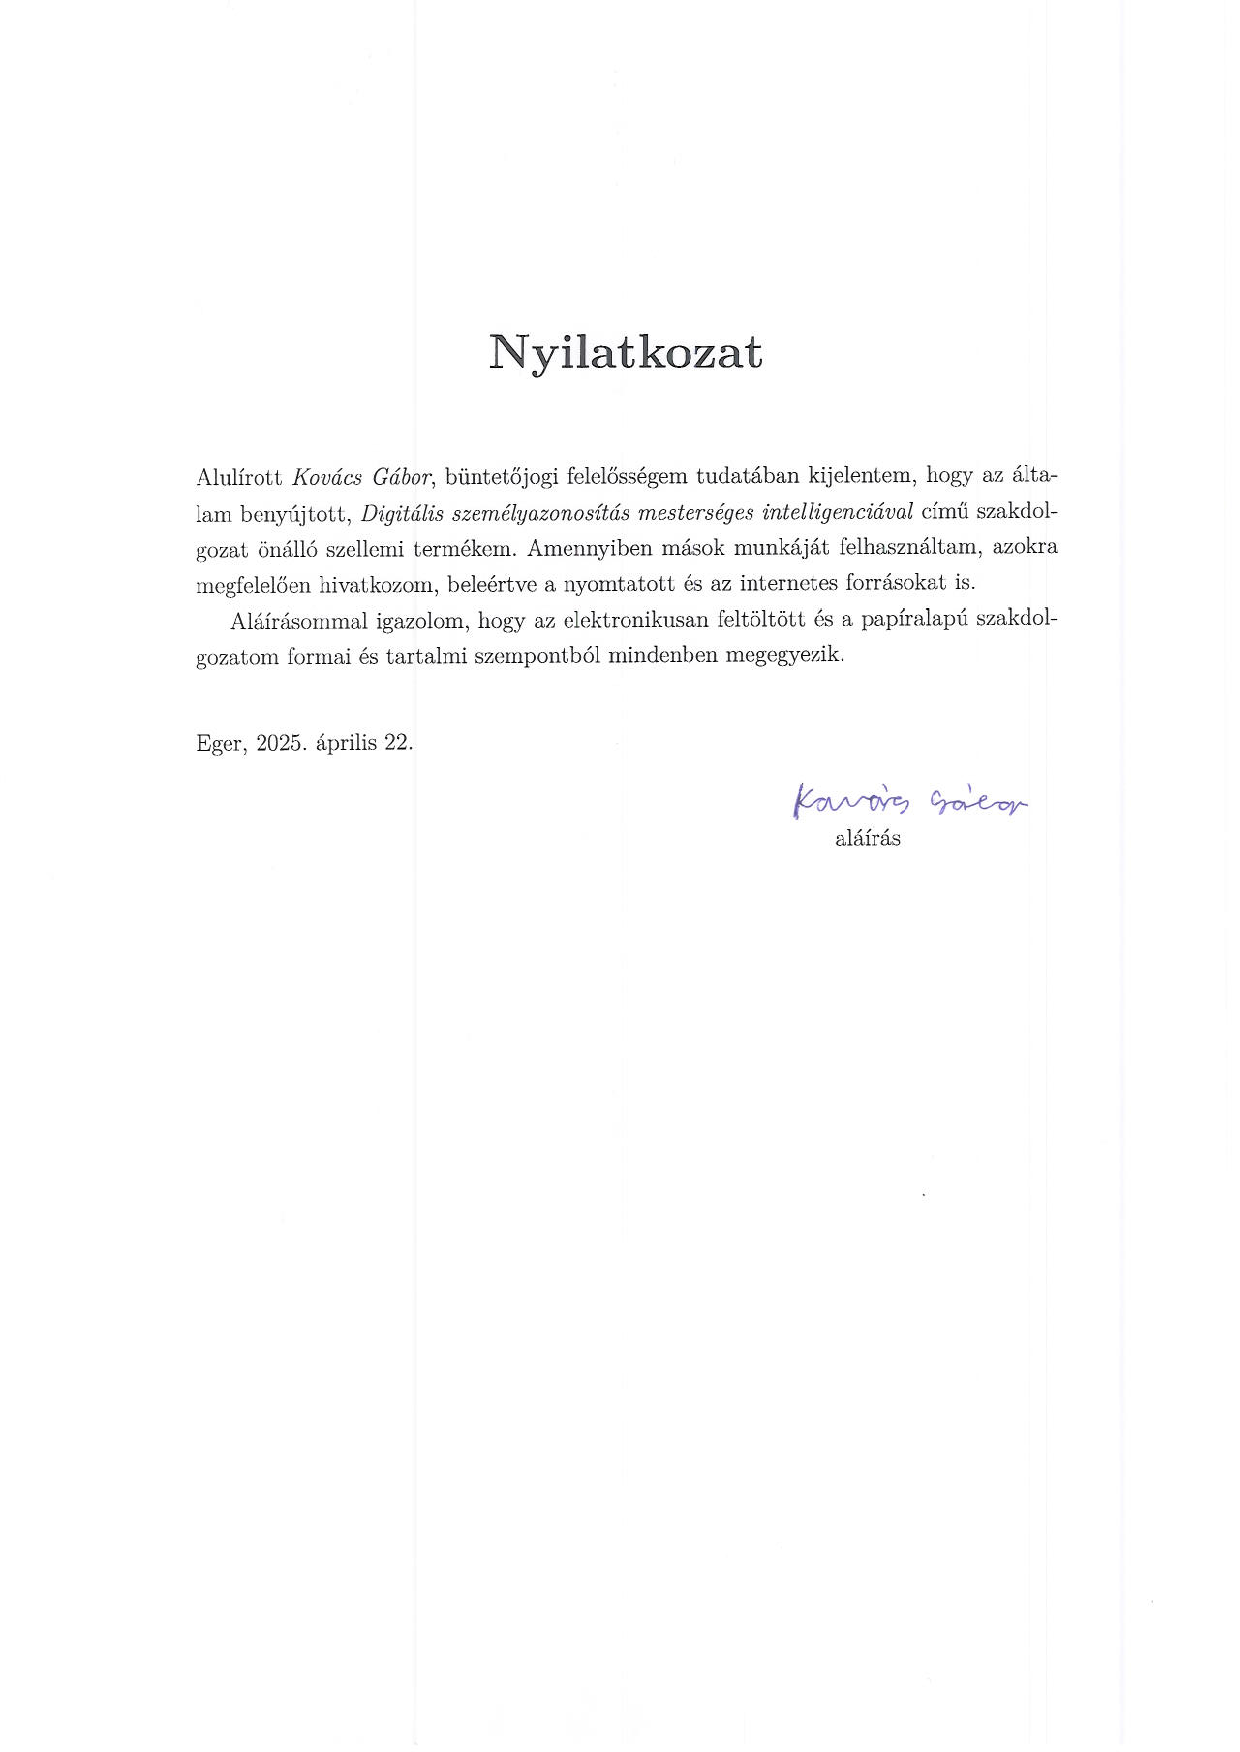
\includepdf{nyilatkozat.pdf}
\end{document}